% Пересечения поверхностной рсчетной сетки.
\newpage
\section*{Глава 3. Пересечение расчетных сеток}                      % выключить номер первой главы
\addcontentsline{toc}{section}{Глава 3. Пересечение расчетных сеток} % но добавить ее в оглавление
\addtocounter{section}{1}                                            % а теперь и счетчик продвинуть
\setcounter{subsection}{0}
\setcounter{figure}{0}
\setcounter{equation}{0}
\setcounter{table}{0}
\setcounter{theorem}{0}
\setcounter{lemma}{0}
\setcounter{definition}{0}

%---------------------------------------------------------------------------------------------------

При моделировании обледенения возникает ряд проблем, связанных с определением пересечения расчетных сеток.

Во время выполнения перестроения поверхностной расчетной сетки может произойти пересечение отдельных ее частей.
Такое пересечение отдельных участков поверхностной расчетной сетки является критическим дефектом, препятствующим проведению дальнейших расчетов.
Таким образом, для обеспечения стабильности моделирования обледенения необходим функционал удаления самопересечения поверхностных расчетных сеток.

Другая проблема связана с пересчетом поля скоростей вокруг поверхностной расчетной сетки после ее перестроения.
Так как геометрия поверхностной расчетной сетки при выполнении расчетов по моделированию обледенения может быть достаточно сложной, к тому же она часто меняется, то поддержка согласованной объемной расчетной сетки в окружающем пространстве для пересчета поля скоростей является слишком ресурсозатратной и может приводить к нестабильности расчетов.
Наиболее целесообразным видится выполнение газодинамических расчетов на расчетной сетке с фиксированной геометрией и сопряжение ее с рассматриваемой поверхностной расчетной сеткой с помощью метода погруженной границы.
Для реализации этого требуется решить задачу определения пересечения поверхностной расчетной сетки и объемной расчетной сетки, а также организовать сопряжение вычислений вблизи области их пересечения.

% Устранение самопересечений
\subsection{Удаление самопересечений расчетной сетки}

В предыдущей главе рассматривались ситуации, когда во время перестроения поверхностной расчетной сетки возникали конфликты из-за сворачивания отдельных ячеек.
В отдельных случаях появление этих конфликтов можно предотвратить с помощью сглаживания нормалей, как это описано в разделе~\ref{sec:tong_method}.
Но наиболее серьезной проблемой, которая может возникнуть при перестроении сетки, является пересечение эволюционирующей поверхности с самой собой, которое будем называть самопересечением \cite{Freylekhman2022GeoIntersect}.
Самопересечение является критическим дефектом сетки, при котором невозможно производить дальнейшие вычисления по моделированию обледенению, поэтому самопересечения необходимо удалять.
В общем случае предотвратить самопересечение невозможно, так как в процессе ледообразования при активном нарастании льда возможно переречение одних ледяных наростов с другими.
Таким образом, для адекватного моделирования обледенения необходимо уметь корректно обрабатывать самопересечения расчетной сетки, чтобы после возникновения самопересечения можно быть продолжить выполнение расчетов.

\subsubsection{Адаптация расчетной сетки}

Все рассмотренные до этого в работе методы перестроения поверхностной расчетной сетки объединяет одно сходство -- они сохраняют количество элементов сетки (узлы, ребра, ячейки) и связи между ними.
Несмотря на некоторые специальные методы по предотвращению конфликтов между гранями сетки и методы сглаживания, после формирования новой поверхности возможно возникновение самопересечений, появление ячеек неправильной формы, а также неравномерное распределение ячеек в сетке по размеру.
Пока опустим самопересечения сетки и будем рассматривать только вопросы, касающиеся формы и размера ячеек.

\begin{figure}[ht]
\centering
\begin{tabular}{ll}
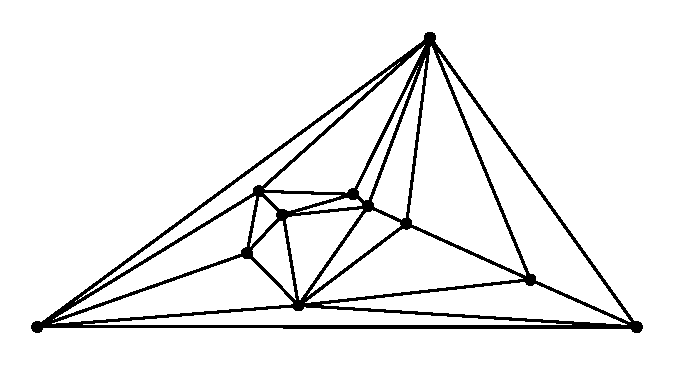
\includegraphics[width=0.35\textwidth]{fig/int_delaunay.pdf}
&
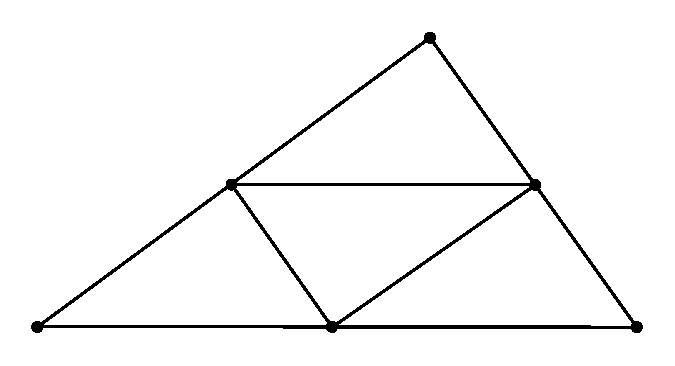
\includegraphics[width=0.35\textwidth]{fig/int_tri_cut.pdf}
\end{tabular}
\singlespacing
\captionstyle{center}\caption{Разбиение ячейки на более мелкие треугольники.}
\label{fig:text_1_int_cut}
\end{figure}

Рассмотрим операцию разбиения ячейки на более мелкие.
В качестве примера такого разбиения можно рассмотреть триангуляцию Делоне по заданному набору точек разбиения внутри ячейки (рис.~\ref{fig:text_1_int_cut} слева) \cite{Rivara2019Delaunay}.
Триангуляция Делоне обладает свойством максимизировать минимальный угол из всех углов треугольников, образованных в результате триангуляции.
Таким образом, триангуляция Делоне позволяет избежать треугольников с очень острыми углами, возникновение которых может привести к нестабильности вычислений на поверхностной расчетной сетке.
Стоит отметить, что разбиение ячейки можно производить с сохранением локальной кривизны сетки, как это показано в \cite{Rakotoarivelo2019Remesh}, но мы этот вариант рассматривать не будем, а будем производить разбиение исключительно в плоскости ячейки.
Если точка разбиения находится не внутри ячейки, а на ее ребре, то разбить придется также вторую инцидентную ячейку этого ребра (если такая есть).
Иногда для уменьшения размера требуется просто разбить ячейку на более мелкие без задания точек разбиения.
В этом случае необходимо следить за качеством результирующих ячеек.
Для определения качества ячейки треугольной формы с узлами $A$, $B$, $C$ можно пользоваться простым критерием качества
\begin{equation}
Q(f) = \frac{4\sqrt{3} S_{ABC}}{|\overline{AB}|^2 + |\overline{BC}|^2 + |\overline{AC}|^2},
\end{equation}
где $Q(f) = 1$ соответствует идеальному случаю равносторонней ячейки, а $Q(f) = 0$ -- худший случай для ячеек с нулевой площадью \cite{Borouchaki2000Remesh}.
Для выполнения разбиения ячейки на более мелкие с сохранением их качества можно просто выполнить разбиение по серединам всех ее сторон (рис.~\ref{fig:text_1_int_cut} справа).

\begin{figure}[ht]
\centering
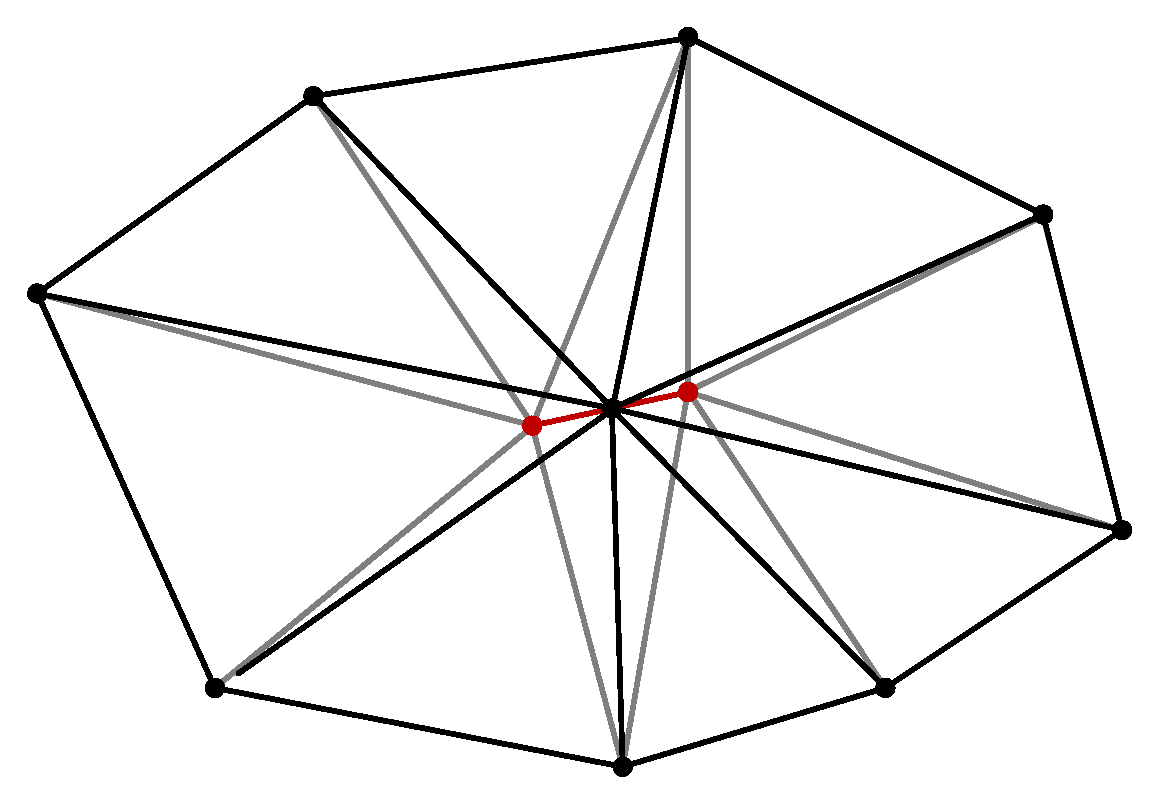
\includegraphics[width=0.4\textwidth]{fig/int_reduce_edge.pdf}
\singlespacing
\captionstyle{center}\caption{Удаление короткого ребра.}\label{fig:text_1_int_reduce_edge}
\end{figure}

Вторая операция, которая необходима для адаптации сетки, связана с огрублением.
Достаточно часто во время выполнения триангуляции по множеству заданных точек могут появляться ячейки с низким показателем качества (у них могут присутствовать либо слишком острые углы, либо близкий к развернутому угол).
Если в ячейке присутствует угол, близкий к развернутому, то избавиться от него поможет разбиение по наибольшей стороне (при этом в качестве точки разбиения следует выбрать основание высоты, опущенной из противолежащего узла).
Если же в треугольнике присутствуют лишь близкие к острым углы, то значит в нем есть слишком короткая сторона, которая может быть удалена.
При удалении ребра $AB$ удаляются обе инцидентные ей грани, узлы $A$ и $B$ соединяются в единый узел $A'$, а все ребра из множества $\mathscr{E}(A) \cup \mathscr{E}(B)$ перенаправляются на узел $A'$ с учетом удаления кратных ребер (рис.~\ref{fig:text_1_int_reduce_edge}).
Эту операцию будем называть стягиванием ребра \cite{Panchal2022Tri}.
Путем применения стягивания наиболее коротких ребер в расчетной сетке можно добиться произвольной степени огрубления.

\subsubsection{Поиск пересекающихся ячеек}

Для поиска самопересечения необходимо определить, какое отношение двух ячеек сетки можно трактовать как самопересечение.
Конечно, простое наличие общих точек у двух ячеек не может служить критерием самопересечения, так как у каждой ячейки есть смежные ячейки (то есть две ячейки могут иметь как общую вершину, так и общее ребро).
Так как смежными могут быть только ячейки, имеющие общие инцидентные объекты (общую инцидентную вершину или общее инцидентное ребро), а все отношения инцидентности зафиксированы в расчетной сетке, то не представляет труда отделить пересечение ячеек по общему инцидентному объекту от самопересечения.

В любом случае для идентификации всех фактов самопересечения сетки требуется проанализировать все пары ячеек и проверить пересечение ячеек в паре (то есть проверить пересечение каждой ячейки с каждой).
Так как прямой перебор всех пар ячеек имеет квадратичную сложность по количеству ячеек в сетке, то его использование на крупных сетках невозможно.
В этом случае целесообразно выполнять поиск пар пересекающихся ячеек с помощью представления множества ячеек в виде специальной древовидной структуры, связанной с ограничением геометрических объектов прямоугольными параллелепипедами в пространстве.

Прямоугольный параллелепипед будем определять как ГМТ\label{abbr:gmt-4} $P = (x, y, z)$ в пространстве, удовлетворяющих следующей системе неравенств:
\begin{equation}\label{eqn:text_1_geo_prim_parallelepiped}
	\left\{
		\begin{aligned}
			& x_l \le x \le x_h \\
			& y_l \le y \le y_h \\
			& z_l \le z \le z_h
		\end{aligned}
	\right.
\end{equation}

Для такого прямоугольного параллелепипеда будем использовать обозначение $Box([x_l, x_h], [y_l, y_h], [z_l, z_h])$.

\begin{definition}
Контейнером произвольного множества точек $M$ в пространстве, который будем обозначать $[M]$, будем называть наименьший прямоугольный параллелепипед, содержащий все эти точки:
\begin{equation}
[M] = Box \left( \left[\min_{P \in M}{P_x}, \max_{P \in M}{P_x}\right],
                 \left[\min_{P \in M}{P_y}, \max_{P \in M}{P_y}\right],
                 \left[\min_{P \in M}{P_z}, \max_{P \in M}{P_z}\right] \right)
\end{equation}
\end{definition}

Контейнер можно рассматривать для произвольного множества точек.
Мы будем его использовать для ячейки расчетной сетки, а также для множества ячеек.
Так как любой треугольник является выпуклой фигурой, то $[ABC] = [\{A, B, C\}]$, то есть для построения контейнера для треугольника достаточно рассмотреть только его вершины.
При поиске пар пересекающихся ячеек будем использовать следующий очевидный факт: если два треугольника пересекаются, то пересекаются и их контейнеры: $ABC \cap A'B'C' \ne \emptyset \implies [ABC] \cap [A'B'C'] \ne \emptyset$.
А значит, что если не пересекаются контейнеры двух треугольников, то не пересекаются и сами треугольники: $[ABC] \cap [A'B'C'] = \emptyset \implies ABC \cap A'B'C' = \emptyset$ (см. рис.~\ref{fig:text_1_int_containers}).

\begin{definition}
Два треугольника $ABC$ и $A'B'C'$ назовем потенциально пересекающимися, если пересекаются их контейнеры $[ABC] \cap [A'B'C'] \ne \emptyset$.
\end{definition}

\begin{figure}[ht]
\centering
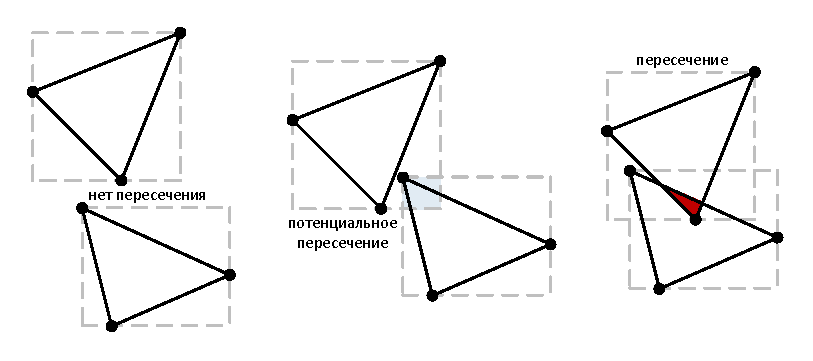
\includegraphics[width=0.65\textwidth]{fig/int_containers.pdf}
\singlespacing
\captionstyle{center}\caption{Потенциальное пересечение треугольников в двумерном варианте.}\label{fig:text_1_int_containers}
\end{figure}

В отличие от анализа пары треугольников на пересечение, проверка на пересечение двух прямоугольных параллелепипедов со сторонами, параллельными координатным осям, является простой операцией.
То есть на первом этапе будем искать пары потенциально пересекающихся ячеек сетки.

Для поиска потенциально пересекающихся ячеек построим иерархическую структуру, которую будем называть деревом облаков треугольников.
Корнем это дерева является контейнер всех ячеек расчетной сетки.
Рассмотрим процедуру разделения контейнера на два более мелких на примере двумерного случая, проиллюстрированного на рис.~\ref{fig:text_1_int_box_tree}.
Путь мы хотим разделить контейнер некоторого множества треугольников ($M$) по горизонтальной прямой на два множества: верхнее ($U$) и нижнее ($D$).
Тогда в верхнее множество попадут все треугольники, лежащие выше прямой, либо пересекающие ее.
Аналогично в нижнее множество попадут все треугольники, лежащие ниже прямой, либо пересекающие ее.
После выделения верхнего и нижнего множества треугольников, для каждого из них строятся свои контейнеры, которые становятся дочерними контейнерами исходного.
После этого получившиеся контейнеры можно делить дальше, используя произвольное направление разбиения ($X$, $Y$, $Z$).

\begin{figure}[ht]
\centering
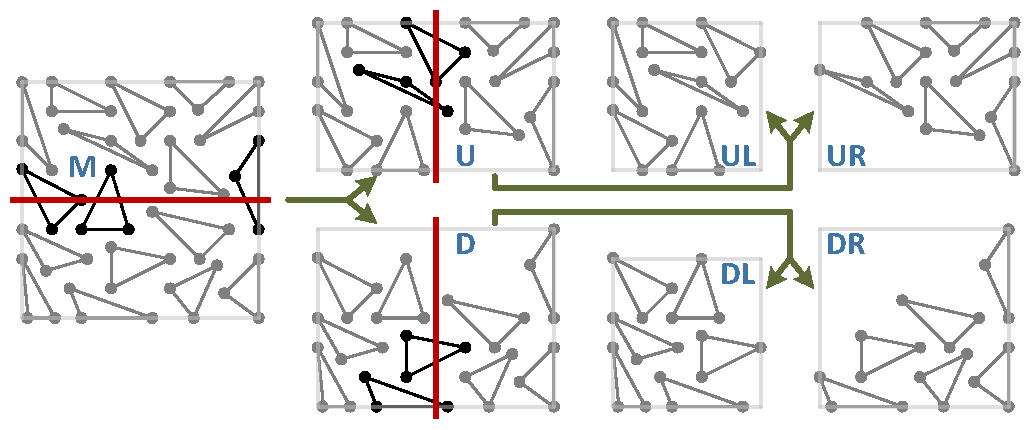
\includegraphics[width=0.85\textwidth]{fig/int_box.pdf}
\singlespacing
\captionstyle{center}\caption{Схема построения дерева контейнеров.}\label{fig:text_1_int_box_tree}
\end{figure}

В частности на рис.~\ref{fig:text_1_int_box_tree} продемонстрировано разбиение исходного контейнера по схеме $[M] \rightarrow \{[U], [D]\} \rightarrow \{\{[UL], [UR]\}, \{[DL], [DR]\}\}$.
Следует заметить, что за одну операцию контейнер можно разбивать на произвольное количество дочерних контейнеров аналогичным образом.
В качестве же направления разбиения контейнера целесообразно выбирать наиболее протяженное (вдоль которого длина контейнера имеет наибольшее значение).
Проводить разбиение контейнеров можно произвольное количество раз, листовые контейнеры в построенном дереве могут содержать произвольное количество треугольников, вплоть до одного треугольника на контейнер.

Введем следующие обозначения.
Пусть $M$ и $M'$ -- два множества треугольников, $K = [M]$ и $K' = [M']$ -- их контейнеры.
Обозначим через $\mathscr{P}(K, K')$ множество пар потенциально пересекающихся треугольников $(T, T')$ таких, что $T \in M$, $T' \in M'$.
Через $\mathscr{C}(K)$ обозначим множество дочерних контейнеров для контейнера $K$.
Тогда множество пар потенциально пересекающихся треугольников может быть вычислено рекурсивно следующим образом:

\begin{equation}
	\mathscr{P}(K, K') =
	\begin{cases}
		\bigcup_{ \substack{ L \in \mathscr{C}(K) \\ L' \in \mathscr{C}(K') } }{ \mathscr{P}(L, L') }, & \text{если } \mathscr{C}(K) \ne \emptyset, \ \mathscr{C}(K') \ne \emptyset \\
		\bigcup_{ L \in \mathscr{C}(K) }{ \mathscr{P}(L, K') },                                        & \text{если } \mathscr{C}(K) \ne \emptyset, \ \mathscr{C}(K') = \emptyset \\
		\mathscr{P}(K', K),                                                                            & \text{если } \mathscr{C}(K) = \emptyset, \ \mathscr{C}(K') \ne \emptyset \\
		\setlength{\jot}{-8pt}
		\begin{split}
			\{ (T, T') : \ & T \in M, \ T' \in M', \\
			               & T \ne T', \ [T] \cap [T'] \ne \emptyset \}
		\end{split},                                                                                   & \text{если } \mathscr{C}(K) = \emptyset, \ \mathscr{C}(K') = \emptyset
	\end{cases}
\end{equation}

Построенное дерево облаков треугольников позволяет существенно сократить количество проверяемых потенциальных пересечений треугольников \cite{Jung2004Int}, так как если $K \cap K' = \emptyset$, $L$ -- дочерний контейнер для $K$, а $L'$ -- дочерний контейнер для $K'$, то $L \cap L' = \emptyset$.
Для поиска всех пар потенциально пересекающихся треугольников из множества всех треугольников расчетной сетки $M$ нужно найти пересечение этого контейнера с самим собой $Int([M], [M])$.

После того, как найдены все пары потенциально пересекающихся треугольников, необходимо проверить, пересекаются ли они на самом деле.

Сначала рассмотрим задачу пересечения треугольника и отрезка в пространстве.
Пусть в пространстве задан треугольник $Tri(A, B, C)$ и отрезок $Segm(P, Q)$.
Для поиска точек пересечения этого треугольника и отрезка требуется найти решение следующей системы уравнений
\begin{equation}\label{eqn:text_1_geo_prim_tri_segm_int}
	\left\{
		\begin{aligned}
			& x_A + (x_B - x_A) \beta + (x_C - x_A) \gamma = x_P + (x_Q - x_P) \alpha \\
			& y_A + (y_B - y_A) \beta + (y_C - y_A) \gamma = y_P + (y_Q - y_P) \alpha \\
			& z_A + (z_B - z_A) \beta + (z_C - z_A) \gamma = z_P + (z_Q - z_P) \alpha
		\end{aligned}
	\right.
\end{equation}
при ограничениях $0 \le \alpha \le 1$, $\beta \ge 0$, $\gamma \ge 0$, $\beta + \gamma \le 1$.

Система уравнений \eqref{eqn:text_1_geo_prim_tri_segm_int} может не иметь решений, может иметь ровно одно решение (если прямая $Line(P, \overline{PQ})$ пересекает плоскость треугольника) либо имеет бесконечное количество решений (если прямая $Line(P, \overline{PQ})$ лежит в плоскости треугольника).

\begin{figure}[ht]
\centering
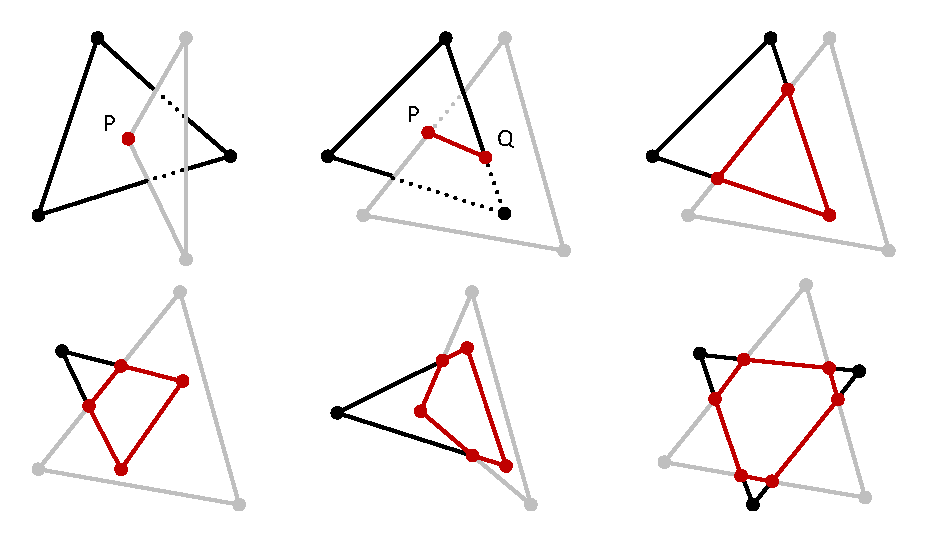
\includegraphics[width=0.7\textwidth]{fig/int_tri_tri.pdf}
\singlespacing
\captionstyle{center}\caption{Пересечение двух треугольников в пространстве.}
\label{fig:text_1_geo_prim_tri_tri}
\end{figure}

Пусть теперь в пространстве заданы два треугольника.
Так как треугольник является выпуклой фигурой, то пересечение двух треугольников либо пусто, либо также является выпуклой фигурой (это может быть плоская фигура с количеством вершин от 1 до 6, см. рис.~\ref{fig:text_1_geo_prim_tri_tri}).

Вершины области пересечения двух треугольников это точки пересечения трех сторон первого треугольника со вторым треугольником и наоборот.
То есть для поиска вершин области пересечения двух треугольников нужно решить 6 задач пересечения треугольника с отрезком в пространстве.

\subsubsection{Обработка пересекающихся треугольников}

После того, как найдены все пары пересекающихся ячеек и области их пересечения, необходимо определить стратегию их устранения.
Все ячейки расчетной сетки можно разделить на три категории (см. рис.~\ref{fig:text_1_int_faces_categories}).

\begin{definition}
Статическими будем называть ячейки, которые не пересекаются ни с какими другими ячейками, и которые должны стать частью итоговой поверхности (будем считать, что в любой момент времени у нас есть возможность указать произвольное количество таких ячеек).
\end{definition}

\begin{definition}
Скрытыми будем называть ячейки, которые не пересекаются ни с какими другими ячейками, но которые не должны стать частью итоговой поверхности (ячейки внутренних петель самопересечения поверхности, которые должны быть удалены).
\end{definition}

\begin{definition}
Ячейками пересечения будем называть ячейки, которые пересекаются с какими-то другими ячейками. 
\end{definition}

\begin{figure}[ht]
\centering
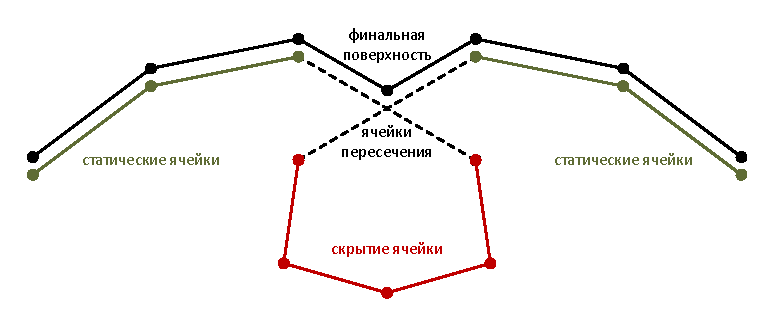
\includegraphics[width=0.65\textwidth]{fig/int_faces_categories.pdf}
\singlespacing
\captionstyle{center}\caption{Категории ячеек при самопересечении сетки в двумерном варианте.}\label{fig:text_1_int_faces_categories}
\end{figure}

\begin{figure}[ht]
\centering
\begin{tabular}{lll}
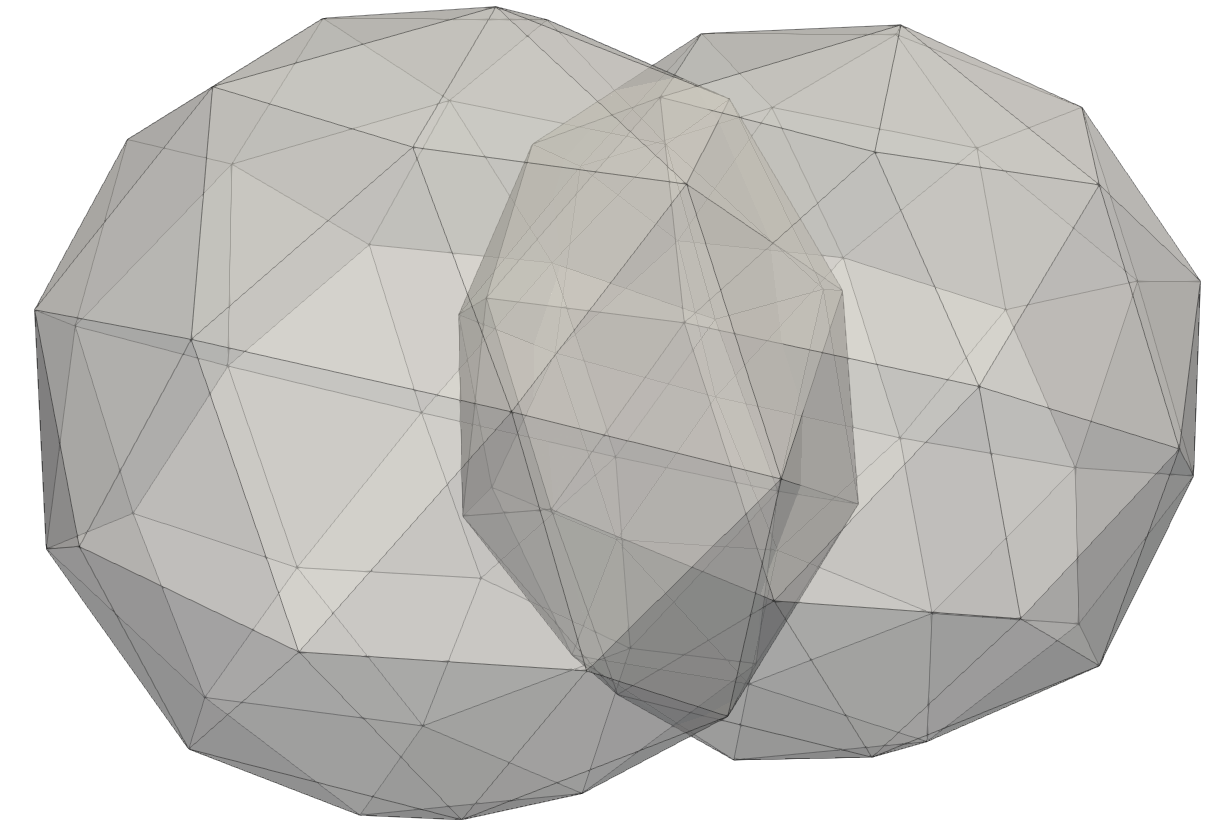
\includegraphics[width=0.3\textwidth]{fig/int_pic_zip_01.png}
&
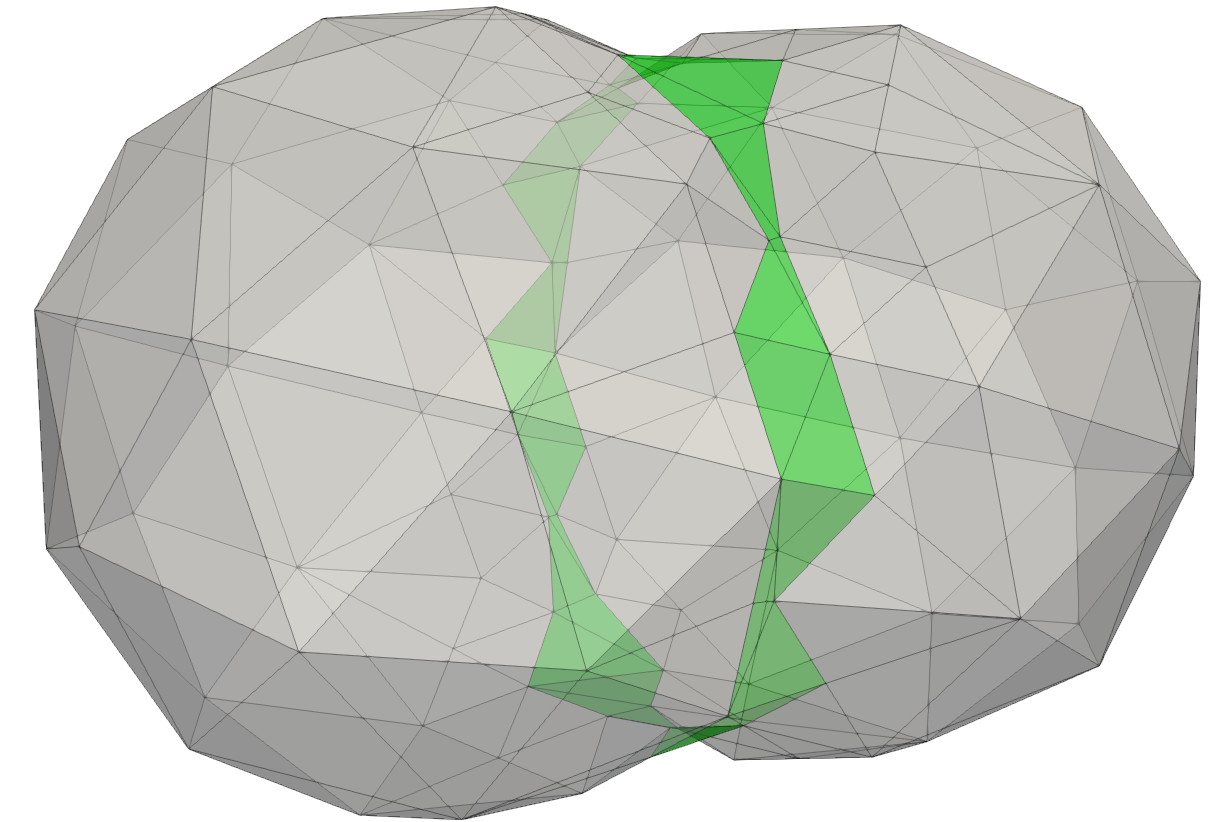
\includegraphics[width=0.3\textwidth]{fig/int_pic_zip_09.png}
&
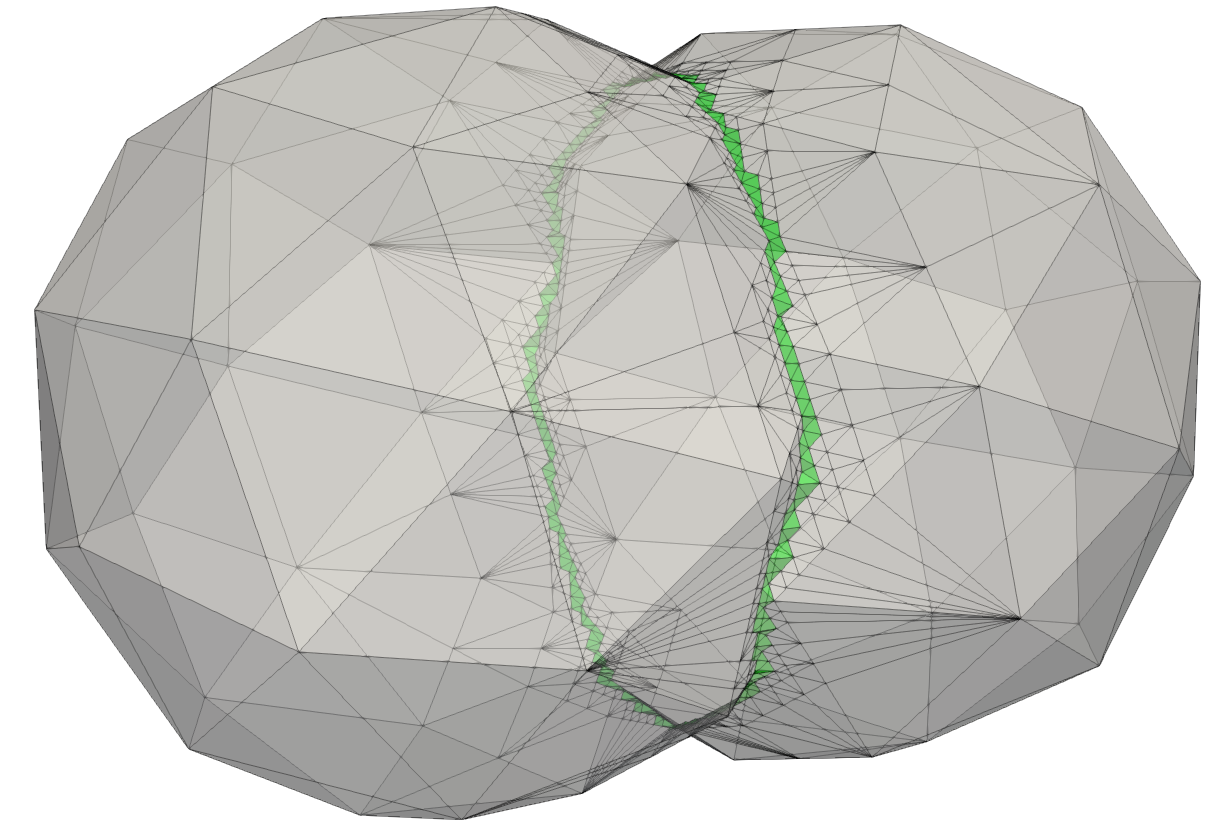
\includegraphics[width=0.3\textwidth]{fig/int_pic_zip_15.png}
\end{tabular}
\singlespacing
\captionstyle{center}\caption{Устранение пересечений двух сфер.}
\label{fig:text_1_int_spheres}
\end{figure}

Одним из подходов к устранению самопересечений сетки является просто удаление всех ячеек пересечения.
После выполнения этой операции сетка распадается на области статических и скрытых ячеек.
При этом скрытые ячейки являются недостижимыми из статических при выполнении обхода ячеек расчетной сетки (если в процессе обхода соседними считаются только ячейки, смежные по ребру).
После удаления из сетки скрытых ячеек расчетная сетка состоит только из статических ячеек, однако требуется добавление новых ячеек для восстановления целостности сетки \cite{Charton2021Repair}.
Такой подход, который мы будем называть методом устранения самопересечений с восстановлением, может применяться для сравнительно простых поверхностей, но в общем случае он не гарантирует получение корректного результата.
В качестве иллюстрации такого способа устранения пересечений на рис.~\ref{fig:text_1_int_spheres} приведен пример работы для устранения пересечений расчетных сеток двух сфер (новые ячейки, появляющиеся при восстановлении сетки отмечены зеленым цветом).
На рис.~\ref{fig:text_1_int_spheres} в середине можно отметить достаточно низкое качество результирующей сетки.
Повысить качество можно с помощью дробления ячеек пересечения.
То есть после поиска всех ячеек пересечения, их необходимо раздробить на более мелкие (как показано на рис.~\ref{fig:text_1_int_cut} справа), после чего повторить процедуру удаления ячеек пересечения и скрытых ячеек и выполнить восстановление сетки.
Процесс дробления ячеек пересечения можно повторять многократно, при этом качество результирующей сетки будет повышаться, как это показано на рис.~\ref{fig:text_1_int_spheres} справа.

При другом подходе устранения самопересечений никакие ячейки из сетки не удаляются, а дробятся на более мелкие по всем точкам пересечения \cite{Skorkovska2018Int}.
Такой подход будем называть методом устранения самопересечений с дроблением.
В качестве примера на рис.~\ref{fig:text_1_int_tri_cut} слева показаны два треугольника, которые пересекаются по отрезку (две точки пересечения).
После выполнения дробления получаем конструкцию, показанную на рис.~\ref{fig:text_1_int_tri_cut} справа.
В общем случае точек, по которым необходимо разбивать ячейку, может быть сколь угодно много, и дробление должно выполняться с помощью выполнения триангуляции по этим точкам, причем некоторые ребра триангуляции должны быть фиксированы.

\begin{figure}[ht]
\centering
\begin{tabular}{ll}
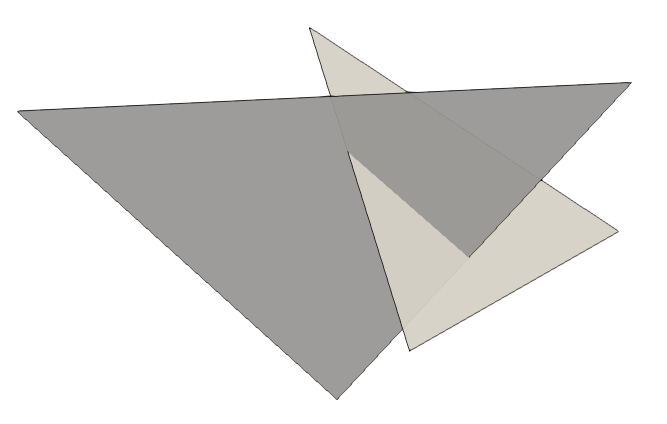
\includegraphics[width=0.35\textwidth]{fig/int_before_cut.png}
&
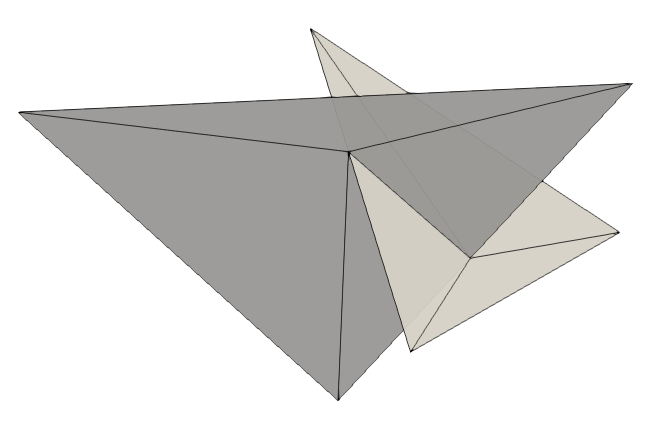
\includegraphics[width=0.35\textwidth]{fig/int_after_cut.png}
\end{tabular}
\singlespacing
\captionstyle{center}\caption{Разбиение треугольника по точкам пересечения.}
\label{fig:text_1_int_tri_cut}
\end{figure}

После дробления ячеек по точкам пересечения, между ячейками сетки могут остаться только следующие виды отношений: две ячейки не имеют общих точек, две ячейки имеют одну общую вершину, две ячейки имеют одно общее ребро.
При этом в сетке появляются ребра, имеющие более двух инцидентных ячеек.
Если наложить на исходную сетку два дополнительных условия, которые могут быть достигнуты с помощью локальных преобразований сетки, то можно добиться достаточно простой структуры сетки (такие сетки будем называть простыми).
Первым условием будем считать отсутствие в сетке совпадающих вершин.
Вторым условием будем считать то, что никакой узел сетки не находится ни в какой другой ячейке.
При выполнении этих двух дополнительных условий можно утверждать, что если ребро имеет более двух инцидентных ячеек, то это количество в точности равно 4, причем эти 4 инцидетные ячейки попарно находятся в одной плоскости.

\begin{figure}[ht]
\centering
\begin{tabular}{lll}
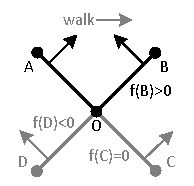
\includegraphics[width=0.25\textwidth]{fig/int_walk_simple.pdf}
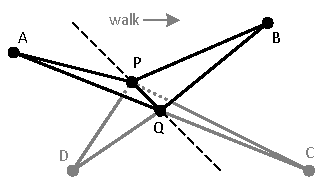
\includegraphics[width=0.3\textwidth]{fig/int_walk_centre.pdf}
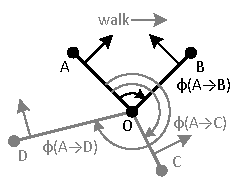
\includegraphics[width=0.3\textwidth]{fig/int_walk_not_simple.pdf}
\end{tabular}
\singlespacing
\caption{Обход внешней поверхности при устранении самопересечений: простая сетка (слева), схема обхода (в центре), общий случай (справа).}
\label{fig:int_walk}
\end{figure}

Для получения результирующей поверхности необходимо избавиться от лишних ячеек, чтобы у каждого ребра вновь осталось ровно по 2 инцидентные ячейки.
Для этого нужно выполнить обход сетки, начиная с любой статической ячейки, считая соседними две ячейки, имеющие общее инцидентное ребро (помечаемые в процессе обхода ячейки попадут в результирующую сетку).
При движении от некоторой ячейки через ребро, имеющее более двух инцидентных ячеек, возникает вопрос выбора ячейки, которая должна войти в результирующую сетку (при этом все остальные ячейки должны быть удалены).

Рассмотрим процедуру выбора следующей ячейки обхода сетки для ребер, имеющих количество инцидентных ячеек, больше двух (рис.~\ref{fig:int_walk}, в центре).
На этом рисунке обозначено направление обхода слева направо, вслед за ячейкой, инцидентной вершине $A$, в результирующую сетку должна войти ячейка, инцидентная вершине $B$.
Рассмотрим эту процедуру для простых сеток, а также для сеток в общем виде.
Для простоты будем рассматривать задачу в проекции на плоскость, перпендикулярную ребру.

Для начала будем считать, что имеет место случай простой сетки (рис.~\ref{fig:int_walk}, слева).
Пусть уже известно, что ячейка, инцидентная вершине $A$, помечена, а ее внешняя нормаль равна $\overline{n}_A$.
Из оставшихся трех ячеек (инцидентных вершинам $B$, $C$, $D$ соответственно) необходимо выбрать только одну для продолжения обхода сетки, а остальные удалить.
Так как сетка у нас простая, то $\angle AOC = \angle BOD = \pi$, а значит $(\overline{n}_A, \overline{OB}) > 0$, $(\overline{n}_A, \overline{OC}) = 0$, $(\overline{n}_A, \overline{OD}) < 0$.
Таким образом, из всех ячеек, необходимо выбрать ту, для которой значение $(\overline{n}_A, \overline{OP})$ максимально.

\begin{figure}[ht]
\centering
\begin{tabular}{ll}
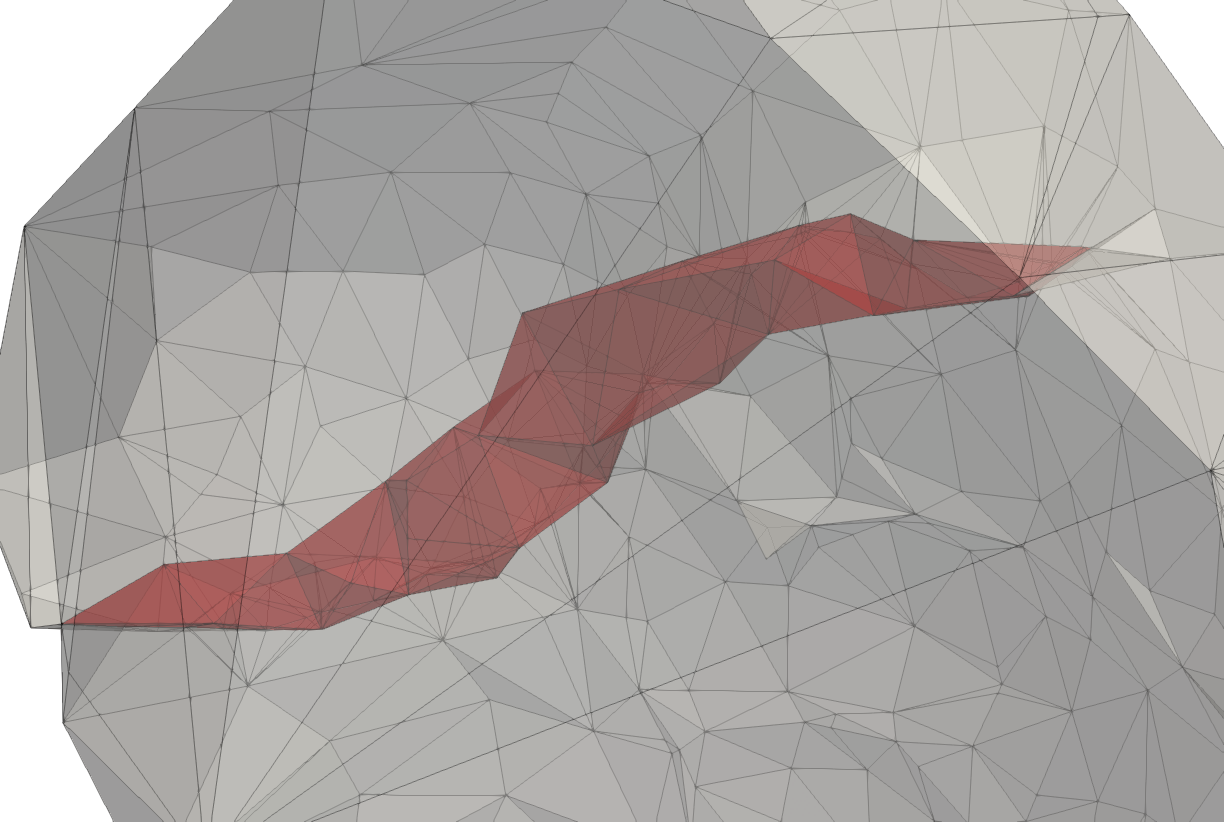
\includegraphics[width=0.45\textwidth]{fig/int_self_intersection_on.png}
&
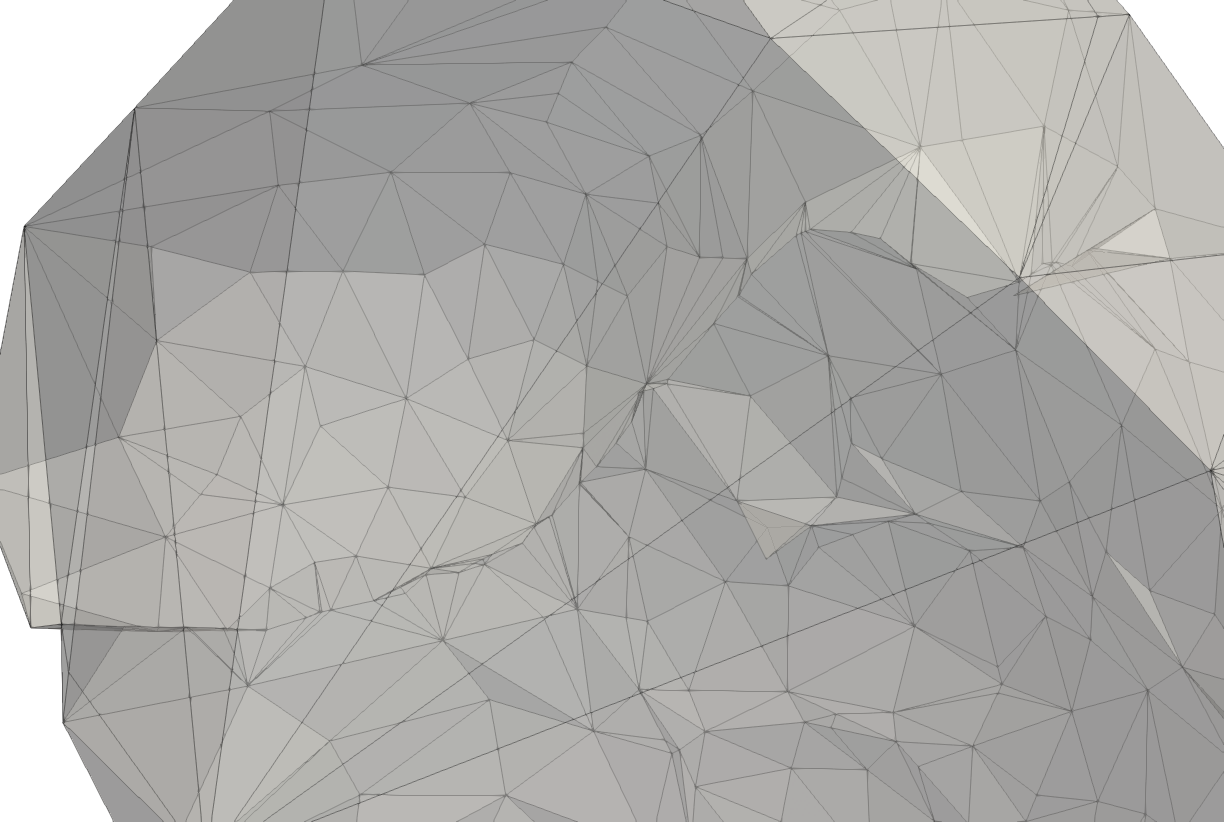
\includegraphics[width=0.45\textwidth]{fig/int_self_intersection_off.png} \\
\\
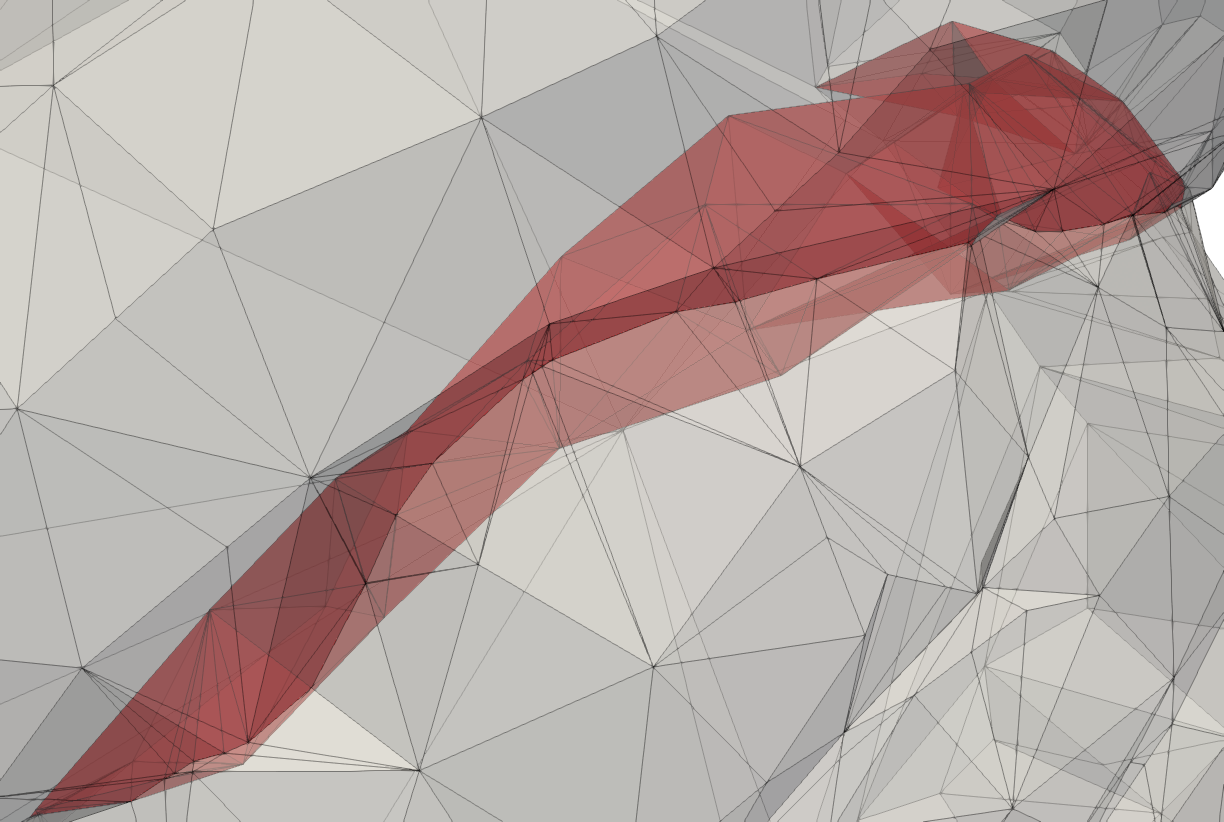
\includegraphics[width=0.45\textwidth]{fig/int_self_intersection_on_2.png}
&
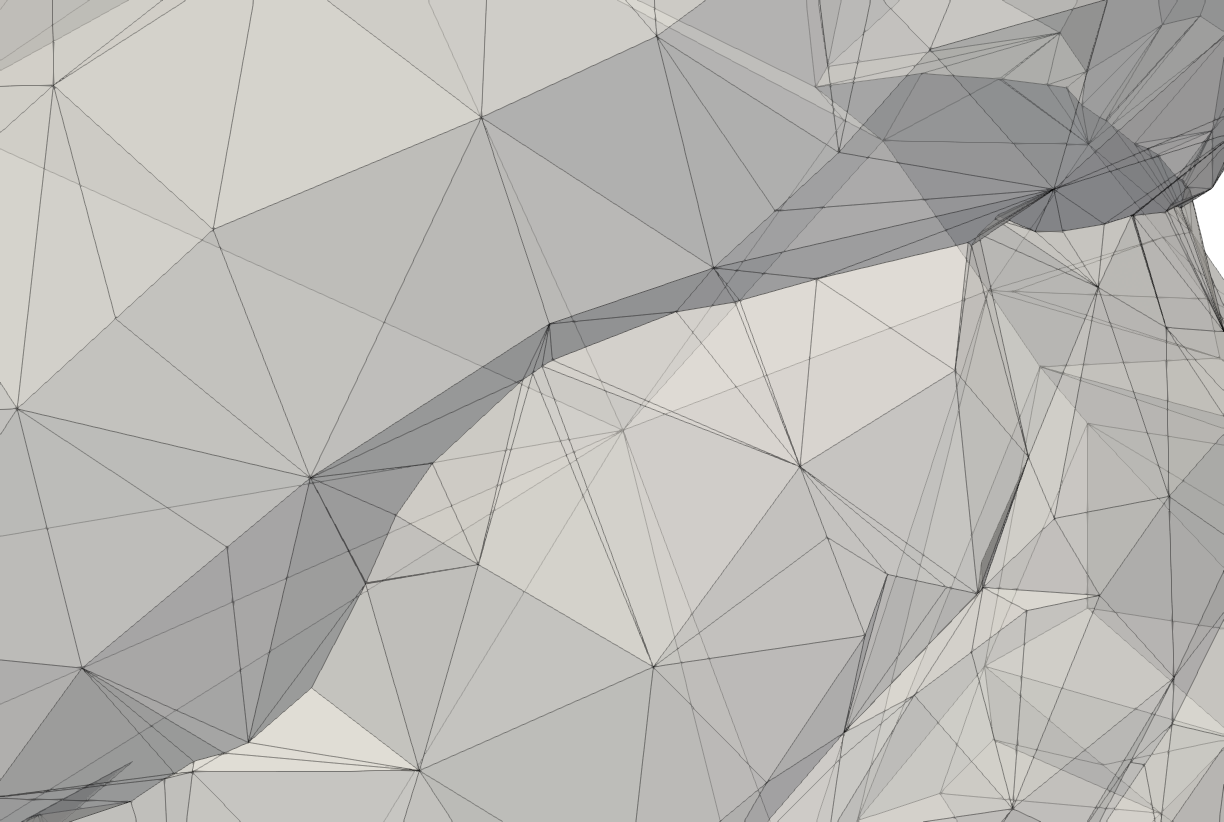
\includegraphics[width=0.45\textwidth]{fig/int_self_intersection_off_2.png}
\end{tabular}
\singlespacing
\captionstyle{center}\caption{Демонстрация удаления самопересечений.}
\label{fig:text_1_int_selfintoff2}
\end{figure}

Теперь рассмотрим расчетную сетку в общем виде.
В этом случае количество ячеек, инцидентных рассматриваемому ребру, может быть произвольным, больше двух, а про значение функции $(\overline{n}_A, \overline{OP})$ сказать ничего нельзя.
Для выбора следующей ячейки для обхода сетки будем поворачивать текущую ячейку вокруг рассматриваемого ребра в направлении $\vec{n}_A$ до совпадения с первой ячейкой (рис.~\ref{fig:int_walk}, справа).
Первая ячейка и должна быть выбрана в качестве следующей для продолжения обхода.
Если через $\phi(A \rightarrow P)$  обозначить угол поворота исходной ячейки в направлении $\overline{n}_A$ до ячеки, инцидентной вершине $P$, то в качестве следующей ячейки для обхода необходимо выбрать ту, для которой $\phi(A \rightarrow B)$ будет минимально.

Объединяя вместе оба рассмотренных случая, получаем критерий выбора следующей для обхода ячейки: должна быть выбрана ячейка, для которой значение показателя $f(P)$ максимально, где $f(P) = (\overline{n}_A, \overline{OP})$ для простых сеток и $f(P) = -\phi(A \rightarrow P)$ в общем случае.

После завершения обхода расчетной сетки все помеченные ячейки считаются ячейками целевой поверхности, а все остальные ячейки должны быть удалены.

На рисунке рис.~\ref{fig:text_1_int_selfintoff2} проиллюстрированы примеры устранения самопересечений сетки в виде скрытых петель.
После удаления скрытых ячеек целевая расчетная сетка снова становится корректной, удовлетворяет соотношениям \eqref{eqn:text_1_remesh3_arch} и может быть использована для дальнейшего моделирования обледенения.

\begin{figure}[ht]
\centering
\begin{tabular}{ll}
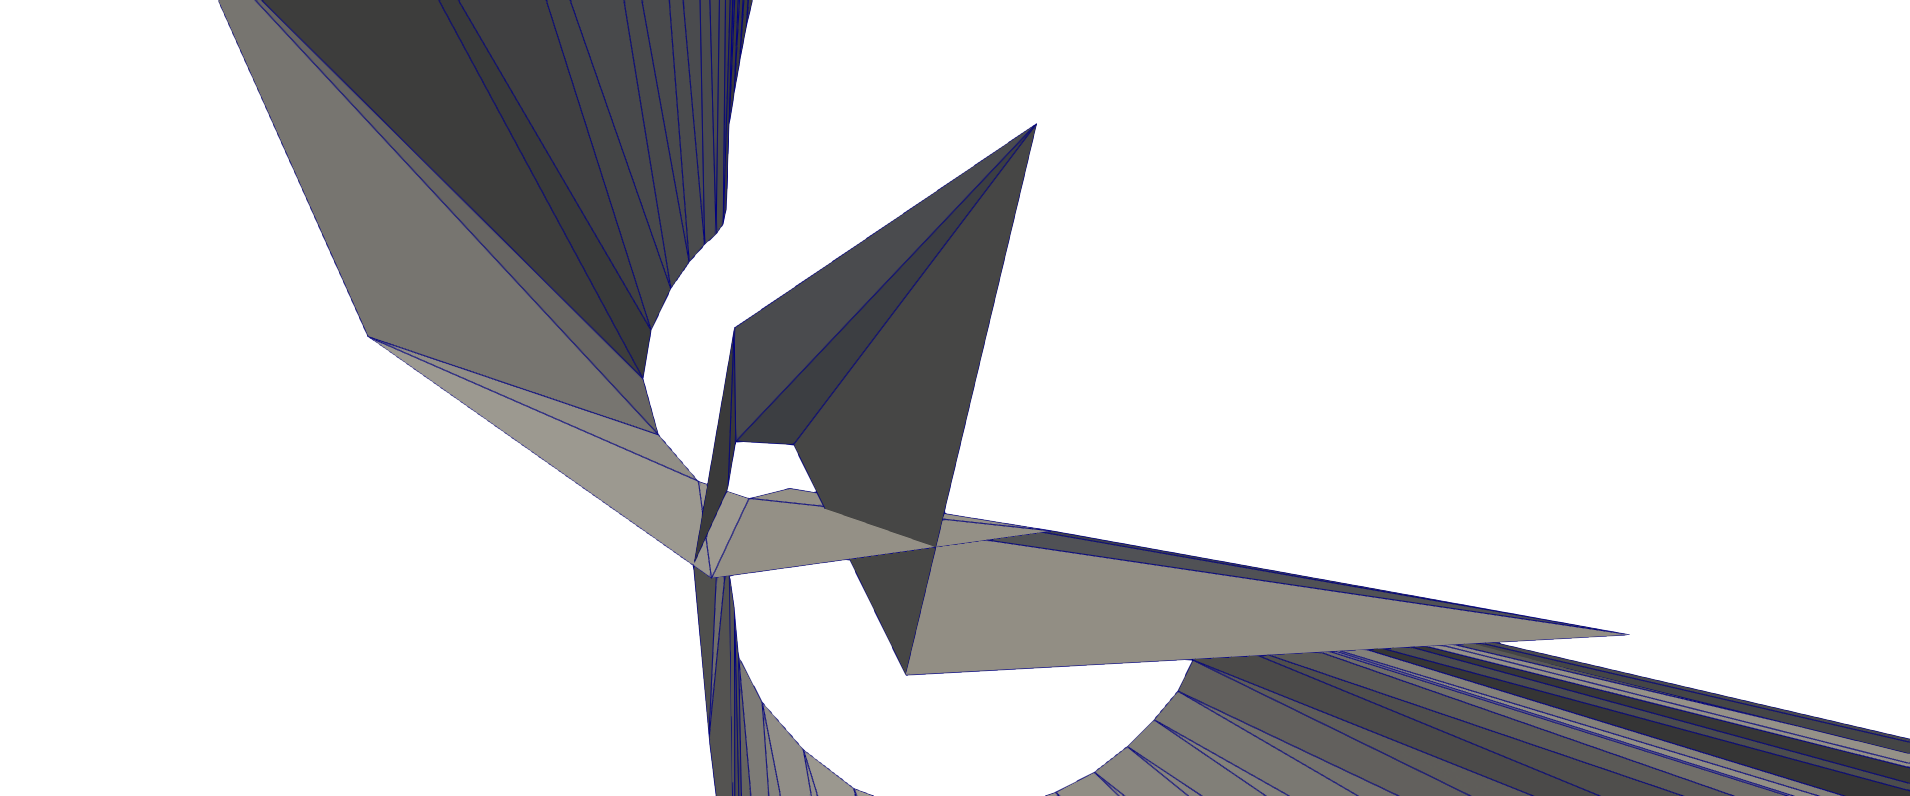
\includegraphics[width=0.45\textwidth]{fig/int_2_remesh_before.png}
&
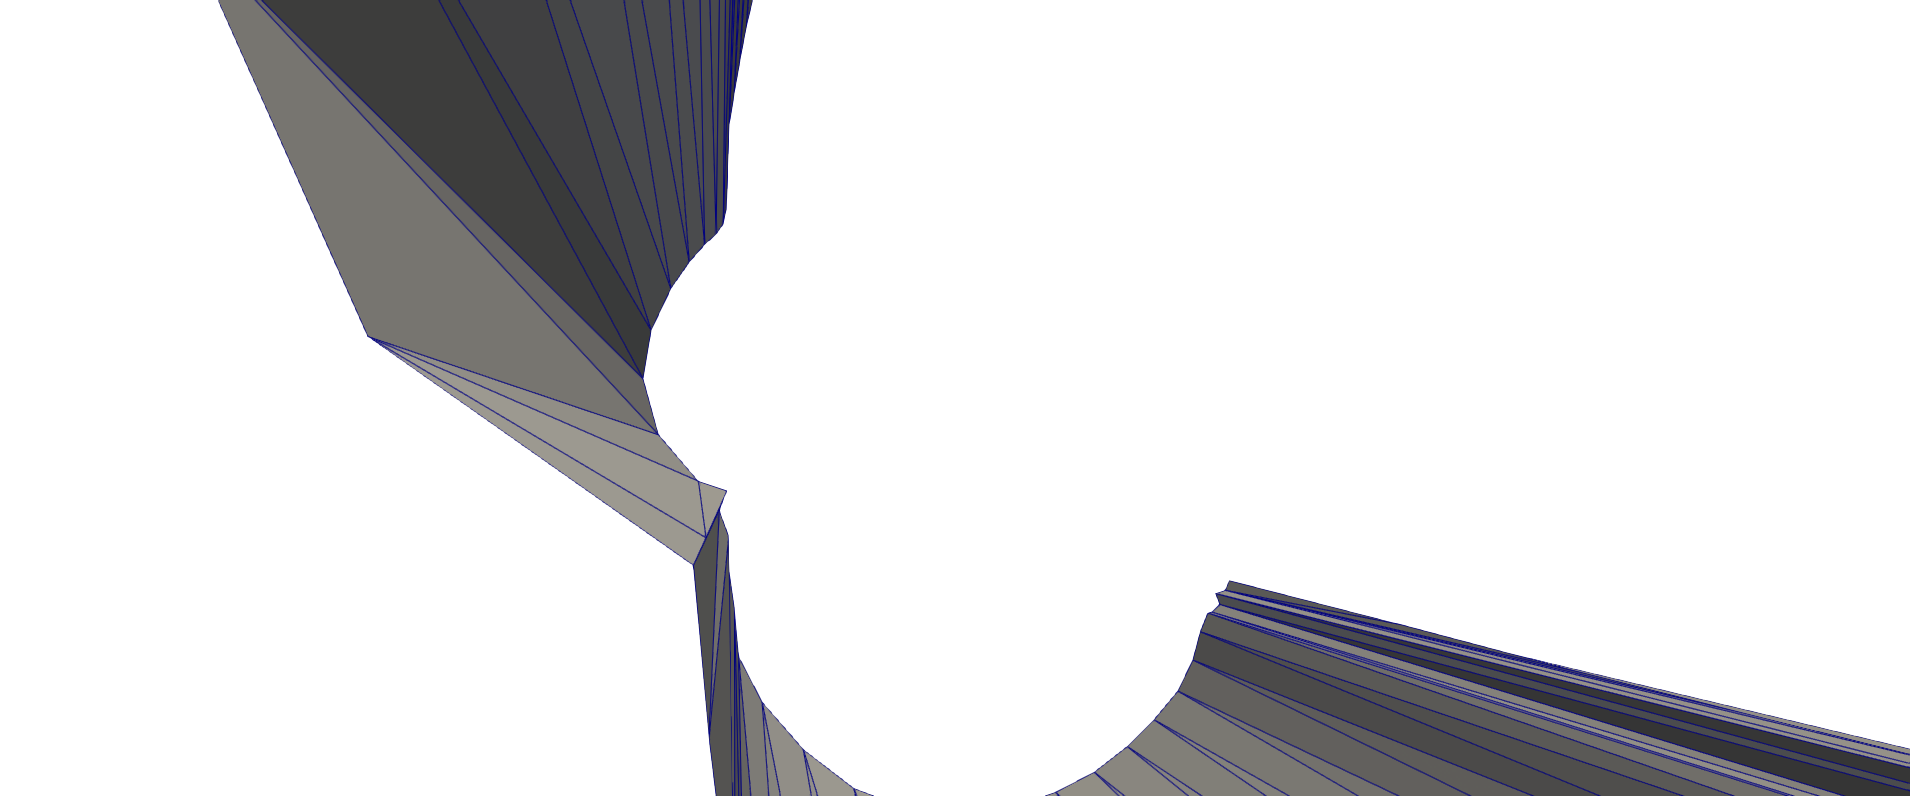
\includegraphics[width=0.45\textwidth]{fig/int_2_remesh_after.png} \\
\end{tabular}
\singlespacing
\captionstyle{center}\caption{Демонстрация удаления самопересечений на псевдодвумерном профиле.}
\label{fig:text_1_int_self_int_demo2}
\end{figure}

На рис.~\ref{fig:text_1_int_self_int_demo2} продемонстрирован пример более наглядного удаления самопересечения на псевдодвумерном профиле (профиль, полученный из двумерного профиля путем представления его в виде трехмерной ленты шириной в одну ячейку).

%---------------------------------------------------------------------------------------------------

\subsection{Сопряжение с газодинамическими решателями}\label{sec:text_1_gas}

При расчете обледенения крайне важным элементом данных является поле скоростей в области, окружающей рассматриваемую поверхность.
Поле скоростей вблизи поверхности влияет на движение жидкой пленки по поверхности, что существенным образом определяет картину обледенения.
Также при использовании модели вторичного увлажнения отскочившие от поверхности капли попадают в свободный поток, и поле скоростей необходимо для расчета траектории их движения и зоны вторичного выпадения.

При выборе газадинамического (CFD\label{abbr:cfd-2}) решателя для сопряжения с расчетным кодом обледения на поверхностной сетке стоит обратить внимание на следующие моменты.
Газодинамический решатель является внешним источником данных для расчетов обледенения поверхности, он запускается довольно редко и вычисленное им поле скоростей используется в неизменном виде несколько сотен или тысяч итераций.
Таким образом, при расчете поля скоростей нет необходимости учитывать турбулентность, а реализацию решателя следует выбрать исходя из требования минимизации времени его работы.
Учитывая это, не ставилась задача выбора оптимального газодинамического решателя \cite{Blazek2015CFD}, а использовались решатели, работающие с трехмерными блочно-структурированными расчетными сетками, ввиду их быстродействия.
Однако, при использовании блочно-структурированных расчетных сеток возникла проблема согласования этих сеток с поверхностью, на которой расчитывается обледенение.
Так как перестроение поверхности в процессе обледенения существенно изменяет ее геометрию, то это приводит к проблемам перестроения объемных сеток для газодинамического решателя.

\subsubsection{Газодинамические решатели}

Приведем краткое описание газодинамических решателей, использованных для вычисления поля скоростей вокруг поверхностной сетки при расчете обледенения.

Рассматривалась система уравнений Эйлера \cite{Kulikovsky2001Gas}
\begin{equation}\label{eqn:text_1_gas_system}
	\frac{\partial}{\partial t} U + \frac{\partial}{\partial x} F + \frac{\partial}{\partial y} G + \frac{\partial}{\partial z} H = 0 \\
\end{equation}

\begin{equation}
U = \begin{pmatrix}
	\rho \\
	\rho u \\
	\rho v \\
	\rho w \\
	E
\end{pmatrix}, \
F = \begin{pmatrix}
	\rho u \\
	\rho u^2 + p \\
	\rho u v \\
	\rho u w \\
	u (E + p)
\end{pmatrix}, \
G = \begin{pmatrix}
	\rho v \\
	\rho u v \\
	\rho v^2 + p \\
	\rho v w \\
	v (E + p)
\end{pmatrix}, \
H = \begin{pmatrix}
	\rho w \\
	\rho u w \\
	\rho v w \\
	\rho w^2 + p \\
	w (E + p)
\end{pmatrix}
\end{equation}

\begin{equation}
	E = \rho \left( \frac{V^2}{2} + e \right), \ V^2 + u^2 + v^2 + w^2, \ e(p, \rho) = \frac{p}{\rho (\gamma - 1)}
\end{equation}

В системе уравнений \eqref{eqn:text_1_gas_system} $U$ -- вектор консервативных переменных, $\rho$ -- давление, $u$, $v$, $w$ -- составляющие вектора скорости вдоль декартовых координат, $p$ -- давление, $e$ -- внутренняя энергия, $E$ -- полная энергия, $\gamma$ -- показатель адиабаты.

Система уравнений \eqref{eqn:text_1_gas_system} решалась на декартовой расчетной сетке с кубическими ячейками с помощью метода конечных объемов путем вычисления потоков консервативных величин $F$ через грани ячейки, перпендикулярные направлению сетки $X$, вектора $G$ через грани ячейки, перпендикулярные направлению сетки $Y$, вектора $H$ через грани ячейки, перпендикулярные направлению сетки $Z$:
\begin{equation}
	U_i^{n + 1} = U_i^n - \frac{\Delta t}{\Delta h} \left( F_{i + \frac{1}{2}} - F_{i - \frac{1}{2}} + G_{j + \frac{1}{2}} - G_{j - \frac{1}{2}} + H_{k + \frac{1}{2}} - H_{k - \frac{1}{2}} \right)
\end{equation}

В первом применяемом решателе для вычисления потоков использовалась противопоточная схема Стегера-Уорминга \cite{Smirnova2018Euler}, в которой потоки получаются следующим образом (на примере потока $F$):
\begin{equation}\label{eqn:text_1_gas_F}
	F_{i + \frac{1}{2}} = F_i^{+}(U_i^n) + F_i^{-}(U_{i + 1}^n)
\end{equation}

\begin{equation}\label{eqn:text_1_gas_F2}
	F^{\pm} = \frac{\rho}{2 \gamma}
	\begin{pmatrix}
		\lambda_1^{\pm} + 2(\gamma - 1)\lambda_2^{\pm} + \lambda_5^{\pm} \\
		(u - a)\lambda_1^{\pm} + 2(\gamma - 1)u\lambda_2^{\pm} + (u + a)\lambda_5^{\pm} \\
		v(\lambda_1^{\pm} + 2(\gamma - 1)\lambda_2^{\pm} + \lambda_5^{\pm}) \\
		w(\lambda_1^{\pm} + 2(\gamma - 1)\lambda_2^{\pm} + \lambda_5^{\pm}) \\
		(H - ua)\lambda_1^{\pm} + (\gamma - 1)V^2\lambda_2^{\pm} + (H + ua)\lambda_5^{\pm}
	\end{pmatrix}
\end{equation}

\begin{equation}
	\lambda_i^{\pm} = \frac{\lambda_i \pm |\lambda_i|}{2}, \ \lambda_1 = u - a, \ \lambda_2 = \lambda_3 = \lambda_4 = u, \ \lambda_5 = u + a, \ H = \frac{E + p}{\rho}
\end{equation}

Во втором применяемом решателе для той же системы уравнений \eqref{eqn:text_1_gas_system} на той же декартовой расчетной сетке с кубическими ячейками использовался метод Годунова \cite{Kulikovsky2001Gas} на базе точного римановского решателя \cite{Borisov2018Riemann} (реализация точного римановского решателя на разных языках программирования доступна в \cite{Toro1999Riemann,riemannvecGithub}).

В качестве третьего решателя (применяемого уже для решения системы уравнений Навье-Стокса) использовался комбинированный метод высокого разрешения RANS/ILES\label{abbr:rans-1}\label{abbr:iles-1} \cite{Bendersky2014RANSILES}, работающий на криволинейных блочно-структурированных расчетных сетках и применяемый для расчета турбулентных течений.
Метод RANS/ILES является комбинацией расчета осредненных по Рейнольдсу уравнений Навье-Стокса (Reynolds averaged Navier-Stokes, RANS) вблизи поверхности, а вдали от нее ILES (implicit LES) -- метода моделирования крупных вихрей (large eddy simulation, LES\label{abbr:les-1}) с неявной подсеточной моделью турбулентности (subgrid scale, SGS\label{abbr:sgs-1}).

\subsubsection{Пересечение поверхностной сетки с подложкой}\label{sec:int_with_undermesh}

Пусть в пространстве определены треугольник $Tri(A, B, C)$ и прямоугольный параллелепипед $Box([x_l, x_h], [y_l, y_h], [z_l, z_h])$.
Требуется определить, имеют ли они общие точки (см. рис.~\ref{fig:text_1_geo_prim_tri_block_intersect}).

\begin{figure}[ht]
\centering
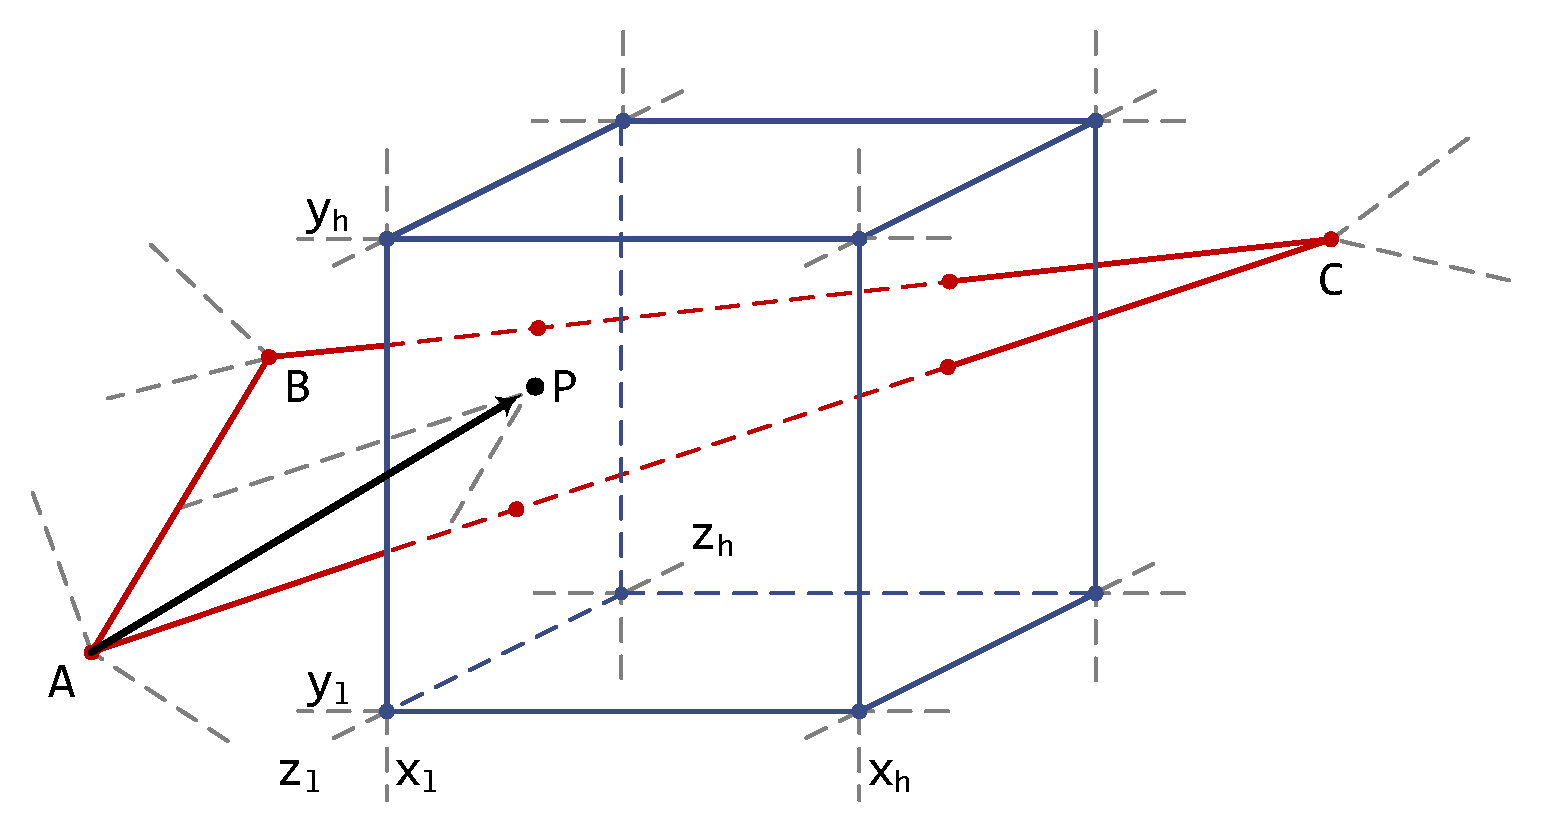
\includegraphics[width=0.7\textwidth]{fig/int_tri_block_intersect.pdf}
\singlespacing
\captionstyle{center}\caption{Пересечение прямоугольного параллелепипеда и треугольника.}
\label{fig:text_1_geo_prim_tri_block_intersect}
\end{figure}

Для решения этой задачи подставим $\overline{P}(\beta, \gamma)$ из \eqref{eqn:text_1_geo_prim_triangle} в систему неравенств \eqref{eqn:text_1_geo_prim_parallelepiped}, получив следующую систему неравенств с двумя переменными $\beta$ и $\gamma$:
\begin{equation}\label{eqn:text_1_geo_prim_1}
	\left\{
		\begin{aligned}
			& x_l \le x_A + \beta (x_B - x_A) + \gamma (x_C - x_A) \le x_h \\
			& y_l \le y_A + \beta (y_B - y_A) + \gamma (y_C - y_A) \le y_h \\
			& z_l \le z_A + \beta (z_B - z_A) + \gamma (z_C - z_A) \le z_h \\
			& \beta \ge 0 \\
			& \gamma \ge 0 \\
			& \beta + \gamma \le 1
		\end{aligned}
	\right.
\end{equation}

Cистема \eqref{eqn:text_1_geo_prim_1} может быть решена методом свертывания конечных систем линейных неравенств \cite{Chernikov1963}.
Для применения метода свертывания систем линейных неравенств неравенства системы \eqref{eqn:text_1_geo_prim_1} необходимо привести к виду $k_{\beta}\beta + k_{\gamma}\gamma + k \le 0$, после чего получим следующую систему неравенств:
\begin{equation}\label{eqn:text_1_geo_prim_2}
	\left\{
		\begin{aligned}
			& (x_B - x_A) \beta + (x_C - x_A) \gamma + (x_A - x_h) \le 0 \\
			& (x_A - x_B) \beta + (x_A - x_C) \gamma + (x_l - x_A) \le 0 \\
			& (y_B - y_A) \beta + (y_C - y_A) \gamma + (y_A - y_h) \le 0 \\
			& (y_A - y_B) \beta + (y_A - y_C) \gamma + (y_l - y_A) \le 0 \\
			& (z_B - z_A) \beta + (z_C - z_A) \gamma + (z_A - z_h) \le 0 \\
			& (z_A - z_B) \beta + (z_A - z_C) \gamma + (z_l - z_A) \le 0 \\
			& -1 \cdot \beta + 0 \cdot \gamma \le 0 \\
			& 0 \cdot \beta + (-1) \cdot \gamma \le 0 \\
			& \beta + \gamma + (-1) \le 0
		\end{aligned}
	\right.
\end{equation}

Cистема неравенств \eqref{eqn:text_1_geo_prim_2} является системой с двумя переменными ($\beta$ и $\gamma$), поэтому после выполнения одного шага свертывания (деформации) она превратится в систему неравенств с одной переменной.
Деформация системы для исключения из нее переменной $\beta$ выполняется следующим образом.
Составляется новая система неравенств, в которую войдут все неравенства системы \eqref{eqn:text_1_geo_prim_2} вида $k_{\gamma} \gamma + k \le 0$, а каждая пара неравенств
\begin{equation}
	\begin{aligned}
		k_{\beta}^1 \beta + k_{\gamma}^1 \gamma + k^1 \le 0 \\
		k_{\beta}^2 \beta + k_{\gamma}^2 \gamma + k^2 \le 0
	\end{aligned}
\end{equation}

в которой коэффициенты при $\beta$ удовлетворяют неравенствам $k_{\beta}^1 < 0$ и $k_{\beta}^2 > 0$, войдет в деформированную систему неравенств в виде
\begin{equation}
	(k_{\gamma}^1 k_{\beta}^2 - k_{\gamma}^2 k_{\beta}^1) \gamma + (k^1 k_{\beta}^2 - k^2 k_{\beta}^1) \le 0. 
\end{equation}

Так как система \eqref{eqn:text_1_geo_prim_2} содержит 9 неравенств, из которых хотя бы в одном коэффициент при $\beta$ нулевой, не более чем в четырех –- положительный, и не более чем в четырех -- отрицательный, то в результате выполнения деформации получим систему, состоящую не более чем из 17 неравенств.
Если деформированная система неравенств с одной переменной имеет решение, то исходные треугольник и прямоугольный параллелепипед имеют общие точки.

\subsubsection{Оптимизация поиска пересечения с подложкой}

Ячейки объемной сетки являются прямоугольными параллелепипедами.
Ячейки поверхностной неструктурированной расчетной сетки являются треугольниками.
Для того, чтобы найти все ячейки объемной сетки, которые пересекаются с поверхностной сеткой, в общем случае необходимо проверить факт пересечения каждой объемной ячейки с каждой поверхностной ячейкой.
В общем случае эта процедура является очень затратной, так как сетки могут содержать большое количество ячеек.
Вместо этого для каждой ячейки поверхностной расчетной сетки сначала будем определять диапазон ячеек объемной сетки, с которыми в принципе возможно пересечение.

Пусть изначально объемная сетка, описывающая область $[X_l, X_h] \times [Y_l, Y_h] \times [Z_l, Z_h]$, размера $S_x \times S_y \times S_z$ разделена на одинаковые ячейки размера $s_x \times s_y \times s_z$, где
\begin{equation}
	n_x = \frac{S_x}{s_x}, \ n_y = \frac{S_y}{s_y}, \ n_z = \frac{S_z}{s_z},
\end{equation}
$n_x$, $n_y$, $n_z$ -- количество ячеек по направлению $X$, $Y$, $Z$ соответственно.

Таким образом, объемная сетка представлена трехмерным массивом ячеек, координаты которых $(x_l, x_h, y_l, y_h, z_l, z_h)$ могут быть вычислены по индексам $(i, j, k)$ в этом трехмерном массиве:

\begin{equation}
	\begin{aligned}
		& x_l(i) = X_l + i s_x, & x_h(i) = X_l + (i + 1) s_x \\
		& y_l(j) = Y_l + j s_y, & y_h(j) = Y_l + (j + 1) s_y \\
		& z_l(k) = Z_l + k s_z, & z_h(k) = Z_l + (k + 1) s_z		
	\end{aligned}
\end{equation}

Для треугольника, являющегося ячейкой поверхностной сетки, вершинами которого являются точки $A$, $B$, $C$, можно найти охватывающий прямоугольный параллелепипед, координаты которого равны

\begin{equation}
	\begin{aligned}
		& \tilde{x}_l = \min(x_A, x_B, x_C), & \tilde{x}_h = \max(x_A, x_B, x_C) \\
		& \tilde{y}_l = \min(y_A, y_B, y_C), & \tilde{y}_h = \max(y_A, y_B, y_C) \\
		& \tilde{z}_l = \min(z_A, z_B, z_C), & \tilde{z}_h = \max(z_A, z_B, z_C)
	\end{aligned}
\end{equation}

Если треугольник пересекает некоторую объемную ячейку, то его охватывающий прямоугольный параллелепипед также пересекает эту ячейку.
То есть для определения пересечения поверхностной ячейки со всеми ячейками объемной сетки достаточно проверить только те ячейки, с которыми пересекается охватывающий прямоугольный параллелепипед рассматриваемого треугольника.
Так как координаты анализируемых параллелепипедов могут быть записаны явно, то можно вычислить диапазоны индексов ячеек, которые требуется проверить на предмет пересечения с треугольником.
Факт пересечения по координате $x$ двух отрезков $[x_l(i), x_h(i)]$ и $[\tilde{x}_l, \tilde{x}_h]$ можно записать в виде системы из двух неравенств
\begin{equation}\label{eqn:text_4_mesh_intersect_eq2}
	\left\{
		\begin{aligned}
			x_l(i) \le \tilde{x}_h \\
			x_h(i) \ge \tilde{x}_l
		\end{aligned}
	\right.
\end{equation}

Преобразовав систему \eqref{eqn:text_4_mesh_intersect_eq2}, и выполнив аналогичные действия для координат по $y$ и $z$, получим диапазоны индексов ячеек объемной сетки

\begin{equation}\label{eqn:text_4_mesh_intersect_diap}
	\left\{
		\begin{aligned}
			\frac{\tilde{x}_l - X_l}{s_x} - 1 \le i \le \frac{\tilde{x}_h - X_l}{s_x} \\
			\frac{\tilde{y}_l - Y_l}{s_y} - 1 \le j \le \frac{\tilde{y}_h - Y_l}{s_y} \\
			\frac{\tilde{z}_l - Z_l}{s_z} - 1 \le k \le \frac{\tilde{z}_h - Z_l}{s_z}
		\end{aligned}
	\right.
\end{equation}

Диапазон индексов из \eqref{eqn:text_4_mesh_intersect_diap} содержит малую долю всех ячеек объемной сетки.

%---------------------------------------------------------------------------------------------------

% Метод погруженной границы.
\subsection{Метод погруженной границы с использованием \mbox{фиктивных} ячеек в трехмерной постановке}\label{sec:text_1_immersed_boundary_method}

При численном решении задач газовой динамики зачастую приходится сталкиваться с областями, обладающими сложной границей (это касается задач обтекания тел со сложной или изменяемой геометрией или расчета потоков внутри областей неправильной формы) \cite{Mahesh2003Turbulent,Ye2020Grid}.
Одним из наиболее ярких примеров проведения расчетов для областей со сложной геометрией является задача формирования ледяного нароста, для которой требуется постоянно пересчитывать аэродинамическое течение в условиях изменения геометрии обтекаемого тела из-за нарастания слоя льда \cite{BourgaultCote2017,Tong2017Remesh,Wright2015LEWICE}.
Для таких областей построение согласованной расчетной сетки может быть крайне требовательной по ресурсам задачей (в некоторых случаях проведение расчетов для таких областей возможно только с использованием неструктурированных или гибридных сеток).
Альтернативой является использование метода погруженной границы (immersed boundary method, IBM\label{abbr:ibm-1}) \cite{Abalakin2018Immersed,Mori2008Immersed,Kim2004Immersed}.
Этот метод позволяет использовать для расчетов несогласованную сетку и даже простую декартову сетку \cite{Clarke1996Cartesian}, что сильно упрощает и ускоряет проведение вычислений.
Применение метода погруженной границы позволяет проводить расчеты на простых структурированных сетках \cite{Farrashkhalvat2003Grid,Rybakov2017Mesh}, что также упрощает имплементацию многопоточных вычислений и распараллеливание расчетных задач и балансировку их выполнения на большом количестве вычислительных узлов суперкомпьютерного кластера \cite{Savin2019RANSILES,Giordano2019Load}.
Единственным тонким моментом метода является выполнение граничных условий на сложной границе, которое достигается путем модификации решаемой системы уравнений \cite{Fadlun2000Immersed}.
Можно выделить два основных подхода к разрешению граничных условий в методах погруженной границы, различающихся по способу выполнения расчетов на границе: задание граничных условий посредством внешних (источниковых) членов \cite{Mittal2005Immersed} и методы, использующие фиктивные (вспомогательные в расчетах) ячейки \cite{Tseng2003Immersed}.

Рассмотрим подробнее метод погруженной границы с использованием фиктивных ячеек \cite{Peter2016Immersed} на примере задачи обтекания тела со сложной геометрией \cite{Rybakov2020GeoIBM}.
Пусть в некоторой области пространства расположено тело, ограниченное сложной границей, представленной неструктурированной поверхностной расчетной сеткой.
В охватывающей тело области пространства строится объемная расчетная сетка, ячейки которой разделяются на следующие три основные класса: внешние, внутренние и граничные.
Внешними ячейками будем называть те ячейки, которые целиком лежат вне тела.
Внутренние ячейки лежат целиком внутри тела, все остальные ячейки пересекают границу тела и являются граничными.
В методе погруженной границы с использованием фиктивных ячеек из граничных ячеек выделяются ячейки, для которых меньшая часть объема находится вне тела, а большая -- внутри тела.
Такие ячейки называются фиктивными.
Это разделение ячеек на классы является первичным и весьма приближенным, так как после коррекции некоторые внутренние ячейки могут быть также переведены в разряд фиктивных (в процессе проведения вычислений должно выполняться следующее требование: соседями внутренних ячеек не могут являться ни граничные, ни внешние ячейки).
На каждой итерации расчетов для фиктивных ячеек требуется выполнить аппроксимацию газодинамических величин (плотность, давление, вектор скорости), чтобы эти фиктивные ячейки могли быть использованы для определения потоков между ними и соседними с ними граничными и внешними ячейками \cite{Vinnikov2007Immersed}.
Таким образом, классификация ячеек объемной сетки является неотъемлемой частью метода погруженной границы.

Аппроксимация газодинамических параметров фиктивных ячеек выполняется на каждой итерации проведения расчетов, после для всех ячеек расчетной сетки кроме внутренних выполняется пересчет потоков между ячейками с использованием любого конечно-объемного метода.
Обработка фиктивных ячеек является основной особенностью рассматриваемого метода, для вычисления газодинамических параметров фиктивных ячеек требуется использование аппроксимации скалярных и векторных величин по данным, взятым из близлежащих точек пространства и поверхности обтекаемого тела.

\subsubsection{Аппроксимации скалярных и векторных величин в методе погруженной границы}

В этом разделе рассматриваются теоретические основы, которые используются при вычислении скалярных и векторных физических величин в фиктивных ячейках расчетной сетки.
Сначала рассмотрим формулу линейной аппроксимации скалярной величины по заданным четырем точкам в пространстве.
Пусть в пространстве определена скалярная величина $\phi = \phi(x, y, z)$ как функция от трех координат.
Пусть известно значение этой величины в четырех точках пространства: $\phi(x_0, y_0, z_0) = \phi_0$, $\phi(x_1, y_1, z_1) = \phi_1$, $\phi(x_2, y_2, z_2) = \phi_2$, $\phi(x_3, y_3, z_3) = \phi_3$.
Требуется выполнить линейную аппроксимацию этой величины, то есть найти представление вида $\phi(x, y, z) = a_0 + a_1x + a_2y + a_3z$, где коэффициенты $a_0$, $a_1$, $a_2$, $a_3$ находятся по известным значениям в четырех точках.
Для двумерного случая задача описана в \cite{Tseng2003Immersed}, и в трехмерном варианте она выглядит аналогично.
Приведем подробное описание задачи для трехмерной постановки.
Для нахождения коэффициентов $a_0$, $a_1$, $a_2$, $a_3$ решается следующая система линейных уравнений:
\begin{equation}\label{eqn:text_1_ibm_sys}
	\left\{
		\begin{aligned}
			a_0 + a_1x_0 + a_2y_0 + a_3z_0 = \phi_0 \\
			a_0 + a_1x_1 + a_2y_1 + a_3z_1 = \phi_1 \\
			a_0 + a_1x_2 + a_2y_2 + a_3z_2 = \phi_2 \\
			a_0 + a_1x_3 + a_2y_3 + a_3z_3 = \phi_3
		\end{aligned}
	\right.
\end{equation}

Система уравнений \eqref{eqn:text_1_ibm_sys} может быть записана в матричной форме в следующем виде:
\begin{equation}
	B_{<0123>}a = \phi_{<0123>},
\end{equation}

где $\phi_{<0123>}$ -- это вектор-столбец $[\phi_0, \phi_1, \phi_2, \phi_3]^T$, $a$ -- вектор-столбец искомых коэффициентов $[a_0, a_1, a_2, a_3]^T$, а матрица $B_{<0123>}$ имеет вид
\begin{equation}\label{eqn:text_1_ibm_B}
	B_{<0123>} =
	\begin{bmatrix}
		1 & x_0 & y_0 & z_0 \\
		1 & x_1 & y_1 & z_1 \\
		1 & x_2 & y_2 & z_2 \\
		1 & x_3 & y_3 & z_3
	\end{bmatrix}
\end{equation}

Отсюда можно найти коэффициенты по формуле $a = B_{<0123>}^{-1}\phi_{<0123>}$.

Следующим шагом рассмотрим аппроксимацию все той же скалярной величины $\phi = \phi(x, y, z)$ с использованием граничного условия Неймана.
Только на этот раз пусть известно ее значение только в трех точках: $\phi(x_1, y_1, z_1) = \phi_1$, $\phi(x_2, y_2, z_2) = \phi_2$, $\phi(x_3, y_3, z_3) = \phi_3$.
Дополнительно в точке $(x_0, y_0, z_0)$ задано условие, соответствующее граничному условию Неймана:
\begin{equation}
	\frac{\partial{\phi}}{\partial{\overline{e}_0}}(x_0, y_0, z_0) = \phi'_0
\end{equation}

где $\overline{e}_0$ -- некоторое направление (граничное условие Неймана задается как производная по нормали к поверхности обтекаемого тела).
При этом будем полагать, что $|\overline{e}_0| = 1$.
Для заданной скалярной величины также требуется выполнить линейную аппроксимацию, то есть найти представление вида $\phi(x, y, z) = a_0 + a_1x + a_2y + a_3z$.
Для двумерного случая задача описана в \cite{Tseng2003Immersed}, приведем ее описание в трехмерном случае.

Пусть компоненты вектора направления $\overline{e}_0$ равны $e_{0,x}$, $e_{0,y}$, $e_{0,z}$ соответственно.
Граничное условие Неймана записывается в следующем виде:
\begin{equation}
	\frac{\partial{\phi}}{\partial{\overline{e}_0}}(x_0, y_0, z_0) = \frac{\partial{\phi}}{\partial{x}}e_{0,x} + \frac{\partial{\phi}}{\partial{y}}e_{0,y} + \frac{\partial{\phi}}{\partial{z}}e_{0,z} = \phi'_0
\end{equation}

Так как известен общий вид аппроксимации функции $\phi(x, y, z) = a_0 + a_1x + a_2y + a_3z$, то и ее частные производные можно выписать в явном виде: $\frac{\partial{\phi}}{\partial{x}} = a_1$, $\frac{\partial{\phi}}{\partial{y}} = a_2$, $\frac{\partial{\phi}}{\partial{z}} = a_3$.
Таким образом, получаем систему из четырех линейных уравнений:
\begin{equation}\label{eqn:text_1_ibm_sys1}
	\left\{
		\begin{aligned}
			& a_1e_{0,x} + a_2e_{0,y} + a_3e_{0,z} = \phi'_0 \\
			& a_0 + a_1x_1 + a_2y_1 + a_3z_1 = \phi_1 \\
			& a_0 + a_1x_2 + a_2y_2 + a_3z_2 = \phi_2 \\
			& a_0 + a_1x_3 + a_2y_3 + a_3z_3 = \phi_3
		\end{aligned}
	\right.
\end{equation}

Система уравнений \eqref{eqn:text_1_ibm_sys1} может быть записана в матричной форме в следующем виде:
\begin{equation}
	B_{<0'123>}a = \phi_{<0'123>},
\end{equation}

где $\phi_{<0'123>}$ -- это вектор-столбец $[\phi'_0, \phi_1, \phi_2, \phi_3]^T$, $a$ -- вектор-столбец искомых коэффициентов $[a_0, a_1, a_2, a_3]^T$, а матрица $B_{<0'123>}$ имеет вид

\begin{equation}\label{eqn:text_1_ibm_B1}
	B_{<0'123>} =
	\begin{bmatrix}
		0 & e_{0,x} & e_{0,y} & e_{0,z} \\
		1 & x_1 & y_1 & z_1 \\
		1 & x_2 & y_2 & z_2 \\
		1 & x_3 & y_3 & z_3
	\end{bmatrix}
\end{equation}

Отсюда получим выражение для коэффициентов линейной аппроксимации $a = B_{<0'123>}^{-1}\phi_{<0'123>}$.

После рассмотрения вопросов, связанных со скалярными величинами, перейдем к векторным физическим величинам.
Для двумерного случая вопрос рассмотрен в \cite{Vinnikov2007Immersed}, однако в трехмерном случае задача несколько сложнее.
При решении задач обтекания тел со сложной геометрией важнейшим вопросом является вычисление значения скорости в фиктивных ячейках, а скорость является векторной величиной.
Итак, рассмотрим векторную величину $\overline{v} = [v_x, v_y, v_z] = [v_x(x, y, z), v_y(x, y, z), v_z(x, y, z)]$, которая задана в трехмерном пространстве как функция от трех координат.
Пусть известны ее значения в трех точках:
\begin{equation}
	\begin{aligned}
		\overline{v}(x_1, y_1, z_1) = \overline{v}_1 = [v_{1,x}, v_{1,y}, v_{1,z}] \\
		\overline{v}(x_2, y_2, z_2) = \overline{v}_2 = [v_{2,x}, v_{2,y}, v_{2,z}] \\
		\overline{v}(x_3, y_3, z_3) = \overline{v}_3 = [v_{3,x}, v_{3,y}, v_{3,z}]
	\end{aligned}
\end{equation}

Дополнительно в точке $(x_0, y_0, z_0)$ задано следующее условие: проекция вектора $\overline{v}_0 = \overline{v}(x_0, y_0, z_0)$ на направление $\overline{e}_0$ равна нулю, а производная составляющей, перпендикулярной направлению $\overline{e}_0$, по этому направлению также равна нулю.
То есть

\begin{equation}
	\left\{
		\begin{aligned}
			& \overline{v}_0 = \overline{v}_0^n + \overline{v}_0^{\tau} \\
			& \overline{v}_0^n \parallel \overline{e}_0 \\
			& \overline{v}_0^{\tau} \perp \overline{e}_0 \\
			& |\overline{e}_0| = 1 \\
			& |\overline{v}_0^n| = 0 \\
			& \frac{\partial{|\overline{v}^{\tau}|}}{\partial{\overline{e}_0}}(x_0, y_0, z_0) = 0 
		\end{aligned}
	\right.
\end{equation}

Требуется определить значение векторной величины в некоторой точке $(x_G, y_G, z_G)$, то есть $\overline{v}_G = \overline{v}(x_G, y_G, z_G)$.
При этом под направлением $\overline{e}_0$ будем подразумевать некоторую нормаль к поверхности обтекаемого тела, для которого выполняется расчет.
Тогда логично называть составляющие вектора $\overline{v}_0^n$ и $\overline{v}_0^{\tau}$ нормальной и тангенциальной составляющими вектора $\overline{v}_0$ соответственно.
Сначала запишем условие равенства нулю нормальной составляющей вектора $\overline{v}_0$, выражающееся в равенстве нулю скалярного произведения $(\overline{v}_0, \overline{e}_0)$. 
Распишем скалярное произведение $(\overline{v}_0, \overline{e}_0)$ покомпонентно:
\begin{equation}
	v_{0,x}e_{0,x} + v_{0,y}e_{0,y} + v_{0,z}e_{0,z} = 0
\end{equation}

Значения $v_{0,x}$, $v_{0,y}$, $v_{0,z}$ нам не известны, поэтому выразим их с помощью линейной интерполяции скалярной величины через точки $P_1 = (x_1, y_1, z_1)$, $P_2 = (x_2, y_2, z_2)$, $P_3 = (x_3, y_3, z_3)$, $P_G = (x_G, y_G, z_G)$:
\begin{equation}
	\left\{
		\begin{aligned}
			v_{0,x} = [1, x_0, y_0, z_0] B_{<G123>}^{-1} v_{<G123>,x} \\
			v_{0,y} = [1, x_0, y_0, z_0] B_{<G123>}^{-1} v_{<G123>,y} \\
			v_{0,z} = [1, x_0, y_0, z_0] B_{<G123>}^{-1} v_{<G123>,z}
		\end{aligned}
	\right.
\end{equation}

Подставляя полученные соотношения для $v_{0,x}$, $v_{0,y}$, $v_{0,z}$ в выражение скалярного произведения $(\overline{v}_0, \overline{e}_0) = 0$, получим:
\begin{equation}
	[1, x_0, y_0, z_0] B_{<G123>}^{-1}
	\left(
		\begin{bmatrix}
			v_{G,x} \\
			v_{1,x} \\
			v_{2,x} \\
			v_{3,x}
		\end{bmatrix} e_{0,x} +
		\begin{bmatrix}
			v_{G,y} \\
			v_{1,y} \\
			v_{2,y} \\
			v_{3,y}
		\end{bmatrix} e_{0,y} +
		\begin{bmatrix}
			v_{G,z} \\
			v_{1,z} \\
			v_{2,z} \\
			v_{3,z}
		\end{bmatrix} e_{0,z}
	\right) = 0
\end{equation}

Введем обозначения $[d_G, d_1, d_2, d_3] = [1, x_0, y_0, z_0] B_{<G123>}^{-1}$, тогда уравнение может быть переписано в следующем виде:
\begin{equation}
	d_G(v_{G,x}e_{0,x} + v_{G,y}e_{0,y} + v_{G,z}e_{0,z}) + d_1(\overline{v}_1, \overline{e}_0) + d_2(\overline{v}_2, \overline{e}_0) + d_3(\overline{v}_3, \overline{e}_0) = 0
\end{equation}

Перепишем это уравнение в виде
\begin{equation}
	v_{G,x}e_{0,x} + v_{G,y}e_{0,y} + v_{G,z}e_{0,z} = Q
\end{equation}

где значение $Q$ может быть вычислено явно следующим образом:
\begin{equation}
	Q = -\frac{d_1(\overline{v}_1, \overline{e}_0) + d_2(\overline{v}_2, \overline{e}_0) + d_3(\overline{v}_3, \overline{e}_0)}{d_G}
\end{equation}

Условие на тангенциальную составляющую $\overline{v}_0^{\tau}$ не будем записывать в явном виде.
Вместо этого будем работать с проекциями вектора $\overline{v}_0$ на векторы, лежащие в плоскости, перпендикулярной вектору $\overline{e}_0$.
Так как компоненты вектора $\overline{e}_0$ известны, то можно без труда найти векторы, перпендикулярные ему.
Это будут, например, следующие векторы: $\overline{f}_1 = [-e_{0,y}, e_{0,x}, 0]$, $\overline{f}_2 = [-e_{0,z}, 0, e_{0,x}]$, $\overline{f}_3 = [0, -e_{0,z}, e_{0,y}]$.

Далее запишем выражения для линейной аппроксимации величин $(\overline{f}_1, \overline{v}_G)$, $(\overline{f}_2, \overline{v}_G)$, $(\overline{f}_3, \overline{v}_G)$ через точки $P_0$, $P_1$, $P_2$, $P_3$ с учетом граничного условия Неймана:
\begin{equation}\label{eqn:text_1_ibm_approx_system}
	\left\{
		\begin{aligned}
			-v_{G,x}e_{0,y} + v_{G,y}e_{0,x} = [1,x_G,y_G,z_G] B_{<0'123>}^{-1}
			\begin{bmatrix}
				0 \\
				-v_{1,x}e_{0,y} + v_{1,y}e_{0,x} \\
				-v_{2,x}e_{0,y} + v_{2,y}e_{0,x} \\
				-v_{3,x}e_{0,y} + v_{3,y}e_{0,x}
			\end{bmatrix} \\
			-v_{G,x}e_{0,z} + v_{G,z}e_{0,x} = [1,x_G,y_G,z_G] B_{<0'123>}^{-1}
			\begin{bmatrix}
				0 \\
				-v_{1,x}e_{0,z} + v_{1,z}e_{0,x} \\
				-v_{2,x}e_{0,z} + v_{2,z}e_{0,x} \\
				-v_{3,x}e_{0,z} + v_{3,z}e_{0,x}
			\end{bmatrix} \\
			-v_{G,y}e_{0,z} + v_{G,z}e_{0,y} = [1,x_G,y_G,z_G] B_{<0'123>}^{-1}
			\begin{bmatrix}
				0 \\
				-v_{1,y}e_{0,z} + v_{1,z}e_{0,y} \\
				-v_{2,y}e_{0,z} + v_{2,z}e_{0,y} \\
				-v_{3,y}e_{0,z} + v_{3,z}e_{0,y}
			\end{bmatrix}
		\end{aligned}
	\right.
\end{equation}

\

В системе уравнений \eqref{eqn:text_1_ibm_approx_system} правые части могут быть непосредственно вычислены, обозначим их $T_{xy}$ , $T_{xz}$ и $T_{yz}$ соответственно и добавим в систему уравнение для выражения $(\overline{v}_G, \overline{e}_0)$.
Получим следующую систему:
\begin{equation}\label{eqn:text_1_ibm_sys3}
	\left\{
		\begin{aligned}
			& v_{G,x}e_{0,x} + v_{G,y}e_{0,y} + v_{G,z}e_{0,z} = Q \\
			& -v_{G,x}e_{0,y} + v_{G,y}e_{0,x} = T_{xy} \\
			& -v_{G,x}e_{0,z} + v_{G,z}e_{0,x} = T_{xz} \\
			& -v_{G,y}e_{0,z} + v_{G,z}e_{0,y} = T_{yz}			
		\end{aligned}
	\right.
\end{equation}

\

В матричной форме система \eqref{eqn:text_1_ibm_sys3} может быть записана следующим образом:
\begin{equation}\label{eqn:text_1_ibm_sys4}
	\begin{bmatrix}
		e_{0,x} & e_{0,y} & e_{0,z} \\
		-e_{0,y} & e_{0,x} & 0 \\
		-e_{0,z} & 0 & e_{0,x} \\
		0 & -e_{0,z} & e_{0,y}
	\end{bmatrix}
	\begin{bmatrix}
		v_{G,x} \\
		v_{G,y} \\
		v_{G,z}
	\end{bmatrix} =
	\begin{bmatrix}
		Q \\
		T_{xy} \\
		T_{xz} \\
		T_{yz}
	\end{bmatrix}			
\end{equation}

Система \eqref{eqn:text_1_ibm_sys4} является переопределенной, и в качестве решения для $\overline{v}_G$ может быть взято его псевдорешение.
Полученные в этом разделе формулы были использованы для аппроксимации скалярных (плотность, давление) и векторных (скорость) физических величин в фиктивных ячейках при реализации метода погруженной границы для обтекания тел со сложной геометрией.

\subsubsection{Реализация метода погруженной границы}\label{sec:text_1_immersed_boundary_method_realization}

Первым шагом реализации метода погруженной границы с фиктивными ячейками является построение структурированной расчетной сетки и выполнение разметки ячеек, которые будут участвовать в вычислительном процессе.

% ----------------- Классификация ячеек. Начало.

Целью разметки (классификации) ячеек является выделение из множества ячеек двух подмножеств: COMMON ячейки -- обычные ячейки для проведения вычислений, GHOST ячейки -- фиктивные ячейки для которых на каждом шаге расчетов требуется выполнять аппроксимацию газодинамических величин.
Для проведения расчетов будем использовать наиболее простой вид сеток -- декартову сетку с кубическими ячейками.
Разметка ячеек производится в две фазы.

\begin{figure}[ht]
\centering
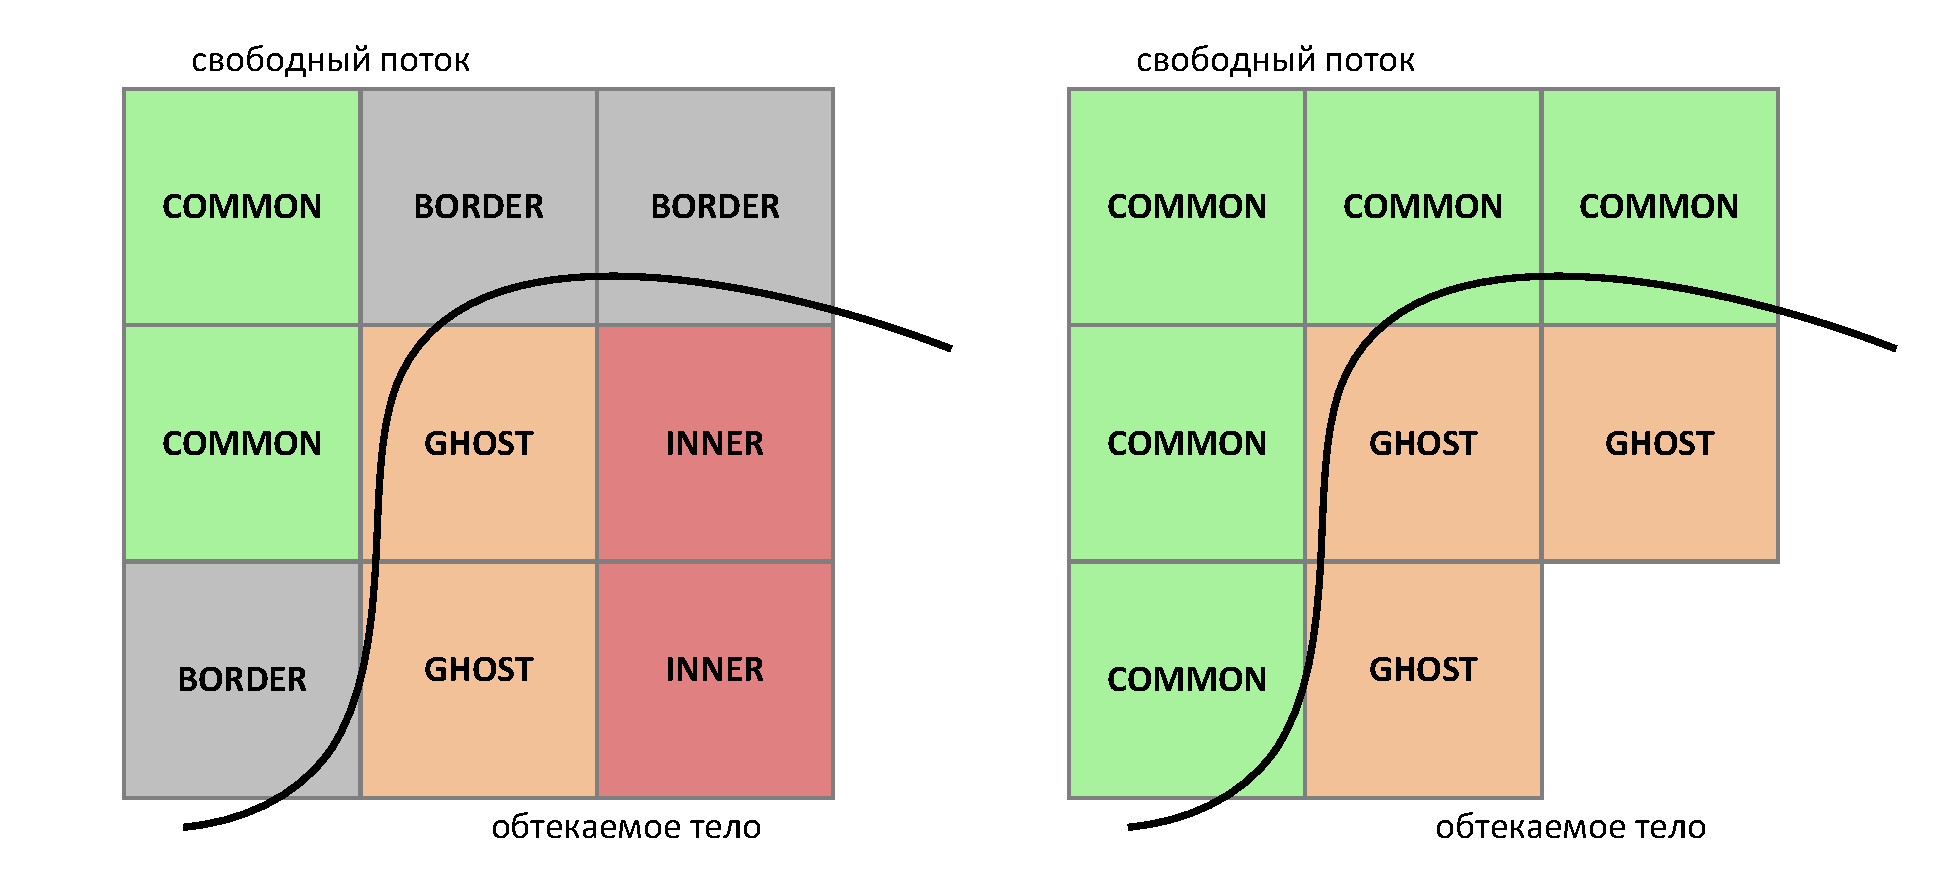
\includegraphics[width=0.8\textwidth]{fig/int_cells_classification.pdf}
\singlespacing
\captionstyle{center}\caption{Классификация ячеек.}
\label{fig:text_1_immersed_boundary_method_class}
\end{figure}

На первой фазе ячейки делятся на 4 типа: к COMMON ячейкам относятся все внешние ячейки, то есть целиком расположенные в расчетной области; к INNER ячейкам относятся все внутренние ячейки, то есть полностью расположенные внутри обтекаемого тела, в них не происходит никаких газодинамических процессов; к BORDER ячейкам относятся граничные ячейки, большая часть объема которых находится вне обтекаемого тела; к GHOST ячейкам относятся фиктивные ячейки, то есть граничные ячейки, большая часть объема которых находится внутри обтекаемого тела (см. рис.~\ref{fig:text_1_immersed_boundary_method_class}, слева).
Ячейками, условно пригодными для расчетов, будем считать COMMON и BORDER ячейки, тогда как ячейки GHOST и INNER относятся скорее к обтекаемому телу. 
Для разграничения ячеек типов BORDER и GHOST вместо оценки доли объема ячейки, лежащей внутри или вне обтекаемого тела, можно использовать более простой критерий: если центр ячейки лежит вне тела, то ячейка помечается как BORDER, в противном случае ячейка помечается как GHOST (это упрощение уместно при том условии, что берется достаточно мелкая расчетная сетка, линейный размер ячеек в которой меньше изломов поверхности).
На рис.~\ref{fig:text_1_mesh_intersect_contour} показан результат разметки ячеек после первой фазы при разном размере объемной сетки.

\begin{figure}[ht]
\centering
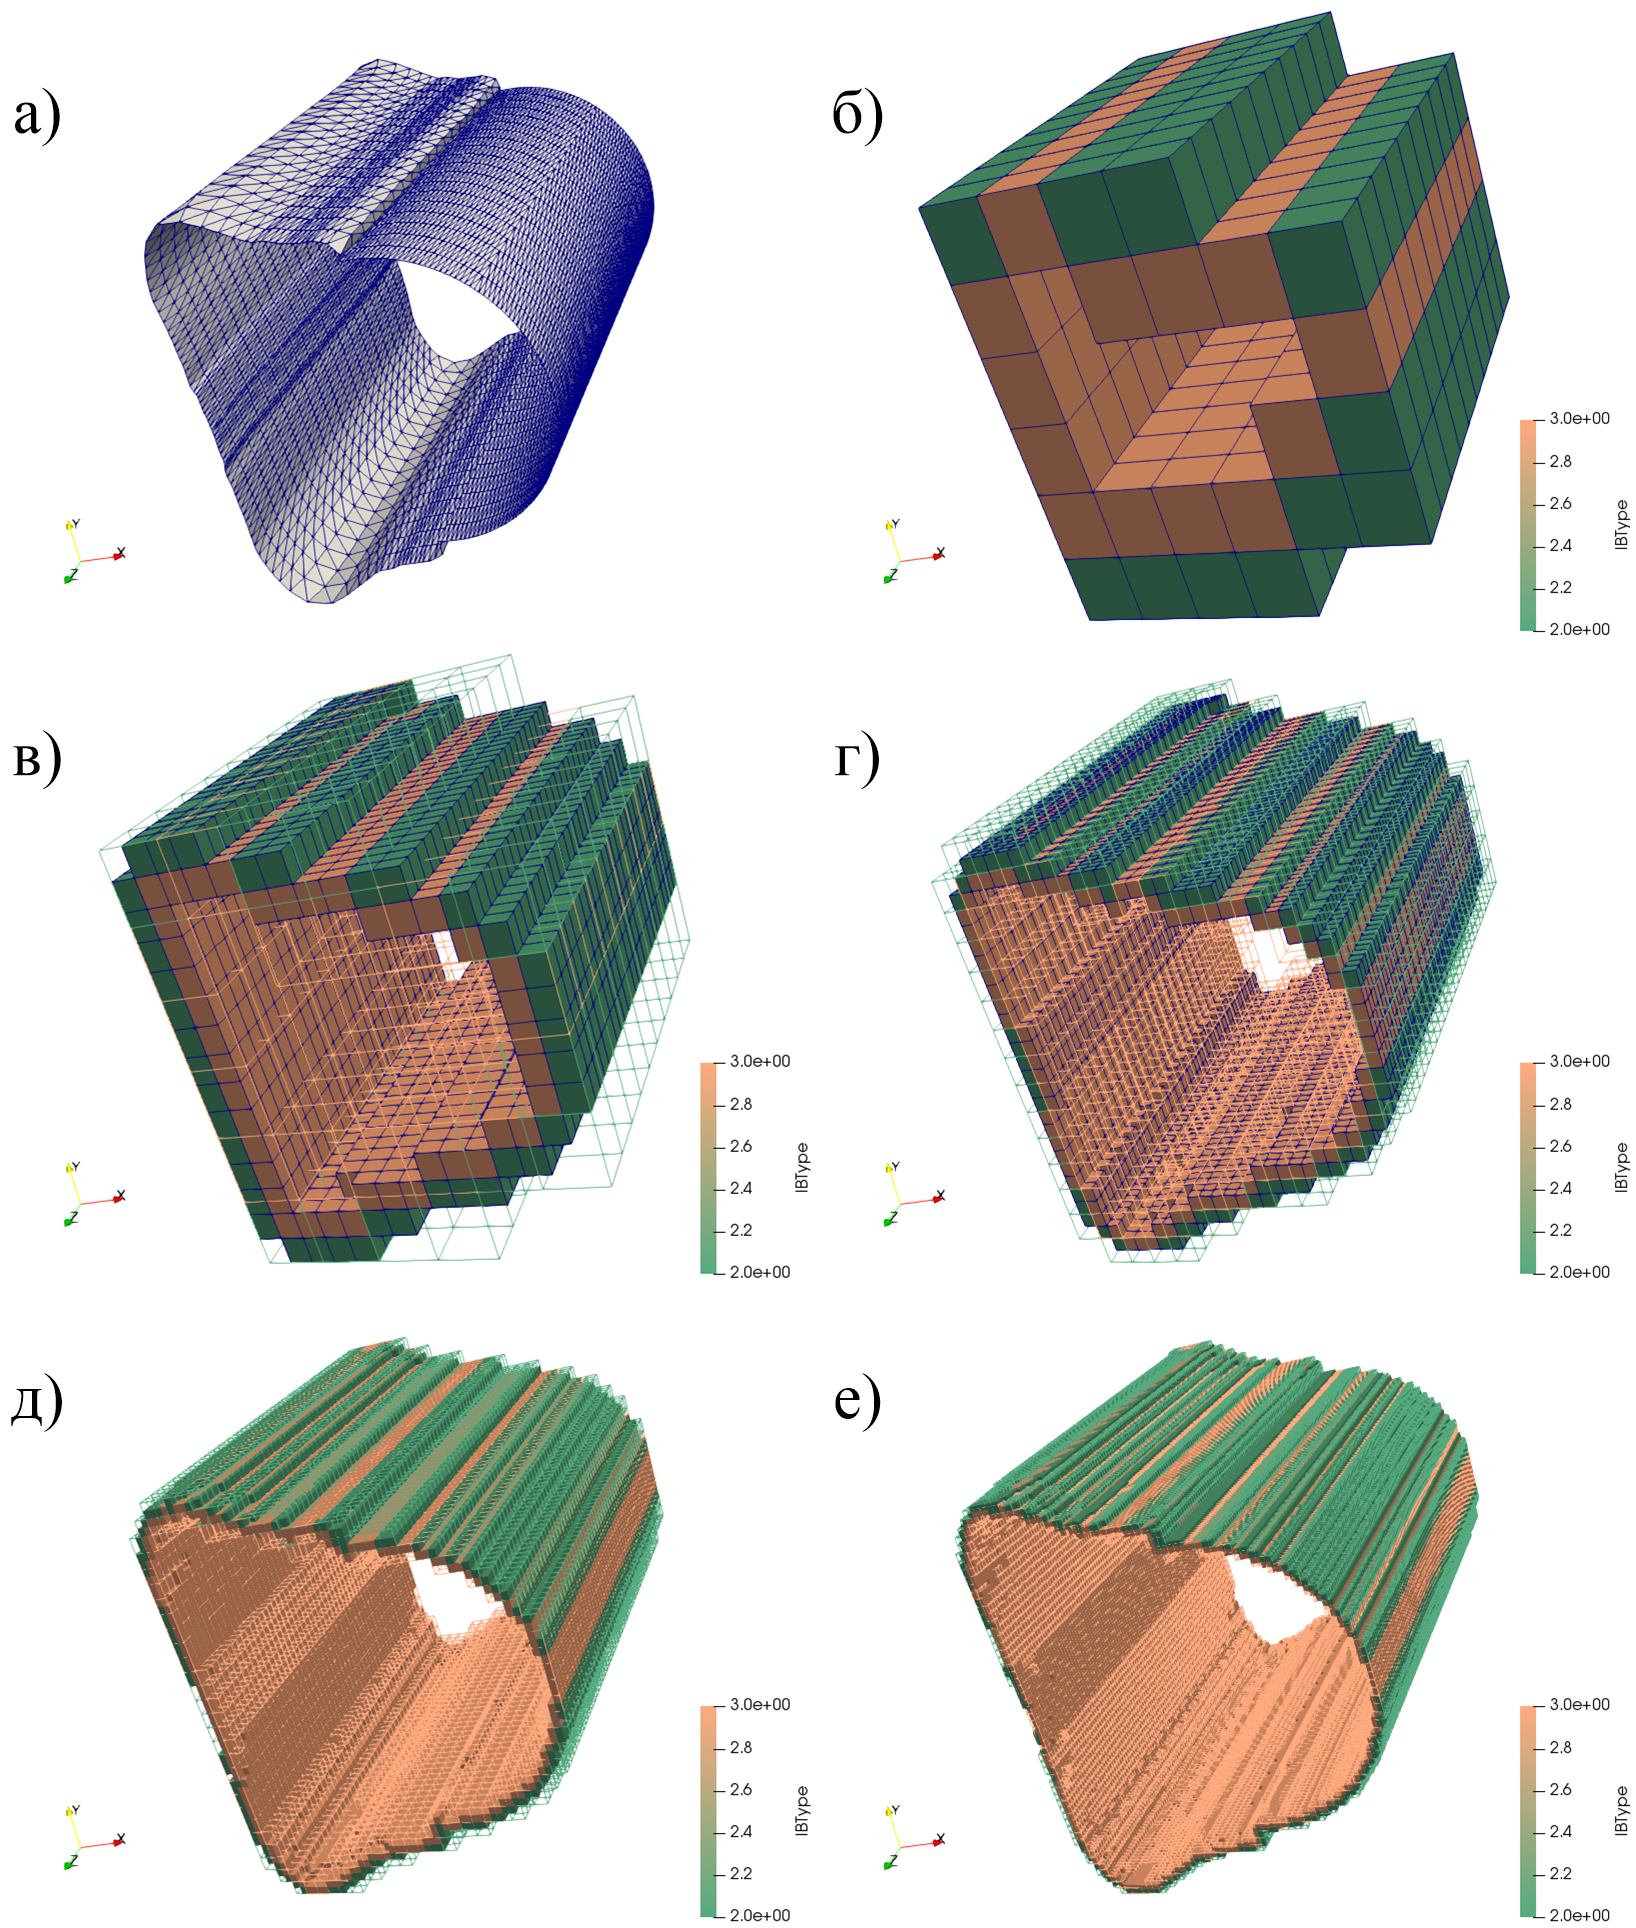
\includegraphics[width=0.6\textwidth]{fig/int_contour.png}
\singlespacing
\captionstyle{center}\caption{Иллюстрация пересечения поверхностной сетки и объемных сеток с разным количеством ячеек. На рисунках цветами обозначены только граничные и фиктивные ячейки объемной сетки (граничные -- зеленые, фиктивные -- бежевые). а) Исходная геометрия поверхностной сетки. б) Размер $10 \times 10 \times 10$. в) Размер $25 \times 25 \times 25$. г) Размер $50 \times 50 \times 50$. д) Размер $100 \times 100 \times 100$. е) Размер $150 \times 150 \times 150$.}
\label{fig:text_1_mesh_intersect_contour}
\end{figure}

После выполнения первой фазы разметки ячеек требуется провести корректировку разметки.
Во время выполнения расчетов конечно-объемным методом для ячеек COMMON и BORDER нужно будет вычислять потоки вещества, импульса и энергии через все границы этих ячеек, а значит все соседи таких ячеек должны содержать газодинамические величины.
Поэтому на фазе коррекции расчетных ячеек все соседи COMMON и BORDER ячеек, которые помечены как INNER, должны быть переквалифицированы в GHOST.
После выполнения этого действия нет больше нужны различать COMMON и BORDER ячейки, а значит все BORDER ячейки можно переквалифицировать в COMMON.
Таким образом, после выполнения фазы коррекции ячеек значения имеют только два типа ячеек: COMMON -- ячейки для которых проводятся газодинамические расчеты, GHOST -- ячейки, для которые газодинамические расчеты не проводятся, но для которых выполняется аппроксимация газодинамических параметров с учетом значений соседних COMMON ячеек и граничных условий (см. рис~\ref{fig:text_1_immersed_boundary_method_class}, справа).

% ----------------- Классификация ячеек. Конец.

На каждой итерации выполнения расчетов для каждой фиктивной ячейки должны быть пересчитаны газодинамические величины на основании данных близлежащих граничных или внешних ячеек (рассматриваются точки, являющиеся центрами таких ячеек), а также точки поверхности обтекаемого тела для аппроксимации граничного условия (для каждой фиктивной ячейки используется ближайшая к ней точка поверхности).
Набор точек, по которым производится аппроксимация данных для фиктивной ячейки, будем называть шаблоном.

Для каждой ячейки существует огромное количество шаблонов даже при использовании простой декартовой расчетной сетки (например, в трехмерном случае общее количество шаблонов для фиктивной ячейки превышает 1000 штук, даже если рассматривать только ближайших соседей).
При использовании же адаптивных локально-измельчающихся сеток \cite{Wackers2011AMR,Zhou2014Refinement,Plas2015Refinement} количество шаблонов резко возрастает, а для таких сеток применение метода погруженной границы представляет особенный интерес.
Многие из этих шаблонов можно не рассматривать изначально (например, это шаблоны, в которые попадают внутренние ячейки или другие фиктивные ячейки), другие шаблоны нужно отсеивать по специальным критериям.
В частности аппроксимация скалярных и векторных величин в GHOST ячейке может быть выполнена, если существуют обратные матрицы $B_{<G123>}^{-1}$ и $B_{0'123}^{-1}$.
Эти матрицы зависят только от выбора соседних COMMON точек, по которым выполняется аппроксимация, а также от направления нормали к поверхности обтекаемого тела в точке поверхности, ближайшей к центру рассматриваемой GHOST ячейки.
Существование обратной матрицы $B_{<G123>}^{-1}$ означает, что точки с индексами $G$, $1$, $2$ и $3$ должны быть точками общего положения, то есть не лежать в одной плоскости.
Существование же обратной матрицы $B_{0'123}^{-1}$ означает, что нормаль из точки поверхности, ближайшей к рассматриваемой GHOST ячейке, не должна быть параллельной плоскости, образованной точками с индексами $1$, $2$ и $3$ (которые не лежат на одной прямой).

На рис.~\ref{fig:text_1_immersed_boundary_method_template} проиллюстрирована схема выбора шаблона аппроксимации газодинамических величин в GHOST ячейке (центр обозначен черной точкой).
Если шаблон выбирается только среди ближайших соседей (индекс ячеек вдоль каждого из направлений структурированной сетки $i$, $j$, $k$ отличается не более чем на единицу), то всего существует 26 ячеек, которые претендуют на включение в шаблон.
Конечно в качестве претендентов рассматриваются только ячейки COMMON, что сразу снижает количество претендентов.
Среди оставшихся ячеек нужно перебрать все комбинации троек ячеек и выбрать любую тройку, для которой существуют обратные матрицы $B_{<G123>}^{-1}$ и $B_{0'123}^{-1}$.
С большой вероятностью среди ближайших соседей возможно найти подходящий шаблон аппроксимации.
В случае же если среди ближайших ячеек не удалось найти тройки COMMON ячеек, которые удовлетворяют всем условиям, то можно рассмотреть более широкую окрестность соседних ячеек для поиска шаблона.

\begin{figure}[ht]
\centering
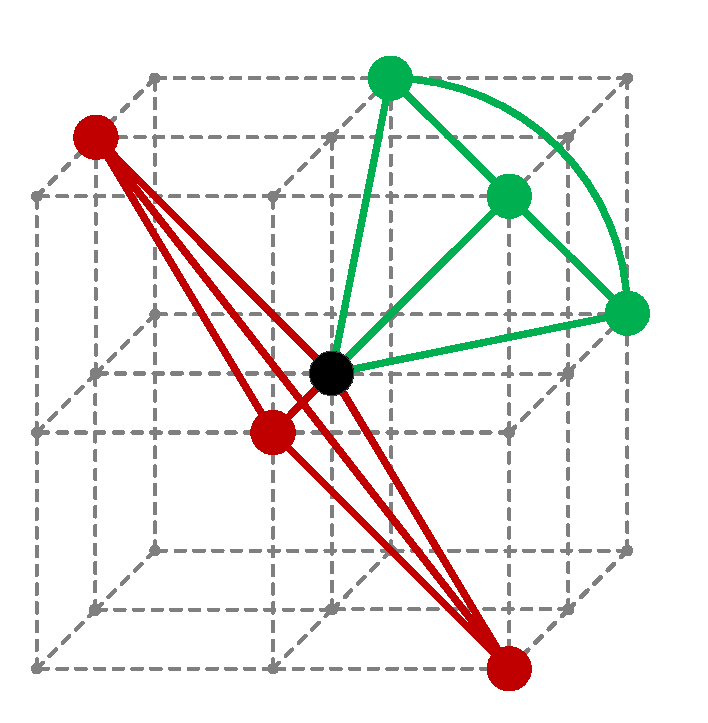
\includegraphics[width=0.3\textwidth]{fig/int_template.pdf}
\singlespacing
\captionstyle{center}\caption{Пример корректного (зеленый) и некорректного (красный) шаблонов относительно матрицы $B_{<G123>}^{-1}$.}
\label{fig:text_1_immersed_boundary_method_template}
\end{figure}

\begin{figure}[ht]
\centering
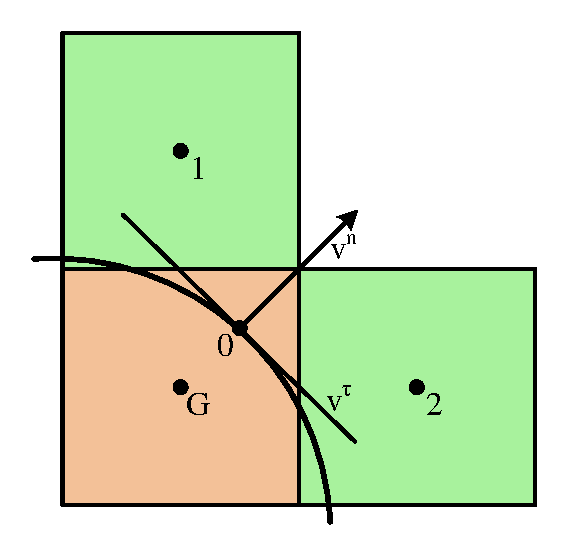
\includegraphics[width=0.3\textwidth]{fig/int_3_points_lin_appr_velocity_2d.pdf}
\singlespacing
\captionstyle{center}\caption{Двумерная иллюстрация аппроксимации скорости в фиктивной ячейке.}
\label{fig:text_1_immersed_boundary_method_2}
\end{figure}

Наибольший интерес представляет аппроксимация векторных величин, а именно аппроксимация вектора скорости в фиктивной ячейке.
Поэтому вопрос аппроксимации скалярных характеристик фиктивных ячеек мы опустим.
На рис.~\ref{fig:text_1_immersed_boundary_method_2} приведена иллюстрация выполнения аппроксимации вектора скорости для двумерного случая (трехмерный случай обрабатывается аналогично).

%\begin{figure}[ht]
%\centering
%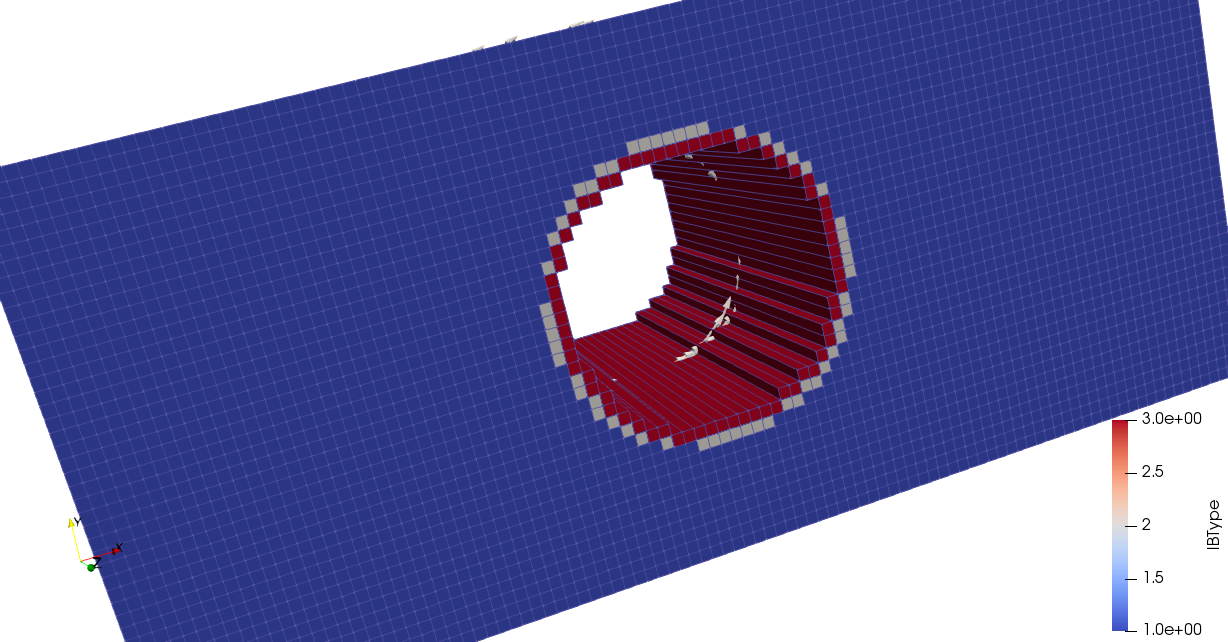
\includegraphics[width=0.7\textwidth]{./pics/text_1_immersed_boundary_method/3d_mesh.png}
%\singlespacing
%\captionstyle{center}\caption{Разбиение расчетной области на внешние, граничные и фиктивные ячейки в задаче обтекания
%цилиндра.}
%\label{fig:text_1_immersed_boundary_method_3}
%\end{figure}

%\begin{figure}[ht]
%\centering
%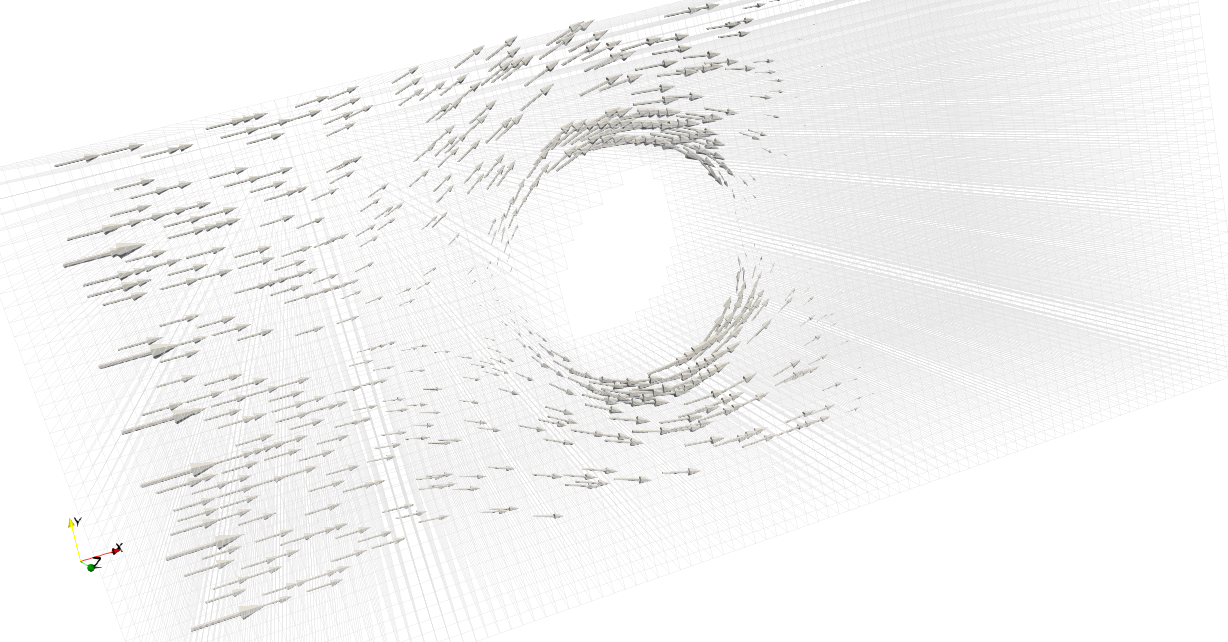
\includegraphics[width=0.7\textwidth]{./pics/text_1_immersed_boundary_method/velocity_field.png}
%\singlespacing
%\captionstyle{center}\caption{Формирование поля скоростей в задаче обтекания цилиндра.}
%\label{fig:text_1_immersed_boundary_method_4}
%\end{figure}

Фиктивная ячейка, центр которой обозначен буквой $G$, большей частью находится внутри обтекаемого тела.
Для выполнения аппроксимации вектора скорости в этой ячейке в качестве шаблона выбраны две соседние граничные ячейки (центры которых обозначены цифрами $1$ и $2$), а также ближайшая к $G$ точка поверхности обтекаемого тела.
Этот шаблон (точки $0$, $1$, $2$) подходит для выполнения аппроксимации, так как никакие две точки в нем не совпадают, а также перечисленные точки не лежат на одной прямой, в дополнение направление нормали, проведенной из точки $0$, не параллельно отрезку, соединяющему точки $1$ и $2$.


Рассмотрим последовательность действий, выполняемых на одной итерации расчетов с использованием метода погруженных границ для схемы Стерега-Уорминга, описанной в разделе~\ref{sec:text_1_gas}.

\begin{enumerate}[noitemsep,topsep=0pt,parsep=0pt,partopsep=0pt]
\item Для всех GHOST ячеек сетки выполнение аппроксимации величин $D = [\rho, u, v, w, p]$ на основе единожды вычисленных шаблонов (подготовку шаблонов и предварительное вычисление матриц мы не рассматриваем, так как это однократное действие, вклад которого в общем процессе расчета стремится к нулю при увеличении времени расчета).
Обозначим это действие функцией \texttt{approximate\_values}.
\item Для всех GHOST и COMMON ячеек сетки получение из вектора величин $D = [\rho, u, v, w, p]$ вектора $U = [\rho, \rho u, \rho v, \rho w, E]$.
Обозначим это действие функцией \texttt{d\_to\_u}.
\item Для всех GHOST и COMMON ячеек сетки вычисление векторов потоков $F^{\pm}$, $G^{\pm}$ и $H^{\pm}$ из \eqref{eqn:text_1_gas_F}, \eqref{eqn:text_1_gas_F2}.
Обозначим это действие функцией \texttt{calc\_fgh}.
\item Для всех COMMON ячеек корректировка вектора $U = [\rho, \rho u, \rho v, \rho w, E]$ с помощью потоков.
Обозначим это действие функцией \texttt{calc\_flows}.
\item Для всех COMMON ячеек обратный пересчет обновленного вектора $U = [\rho, \rho u, \rho v, \rho w, E]$ в вектор $D = [\rho, u, v, w, p]$.
Обозначим это действие функцией \texttt{u\_to\_d}.
\end{enumerate}

Схема выполнения расчетов продемонстрирована на рис.~\ref{fig:text_4_ibm_immersed_boundary_method_cheme}.

\begin{figure}[ht]
\centering
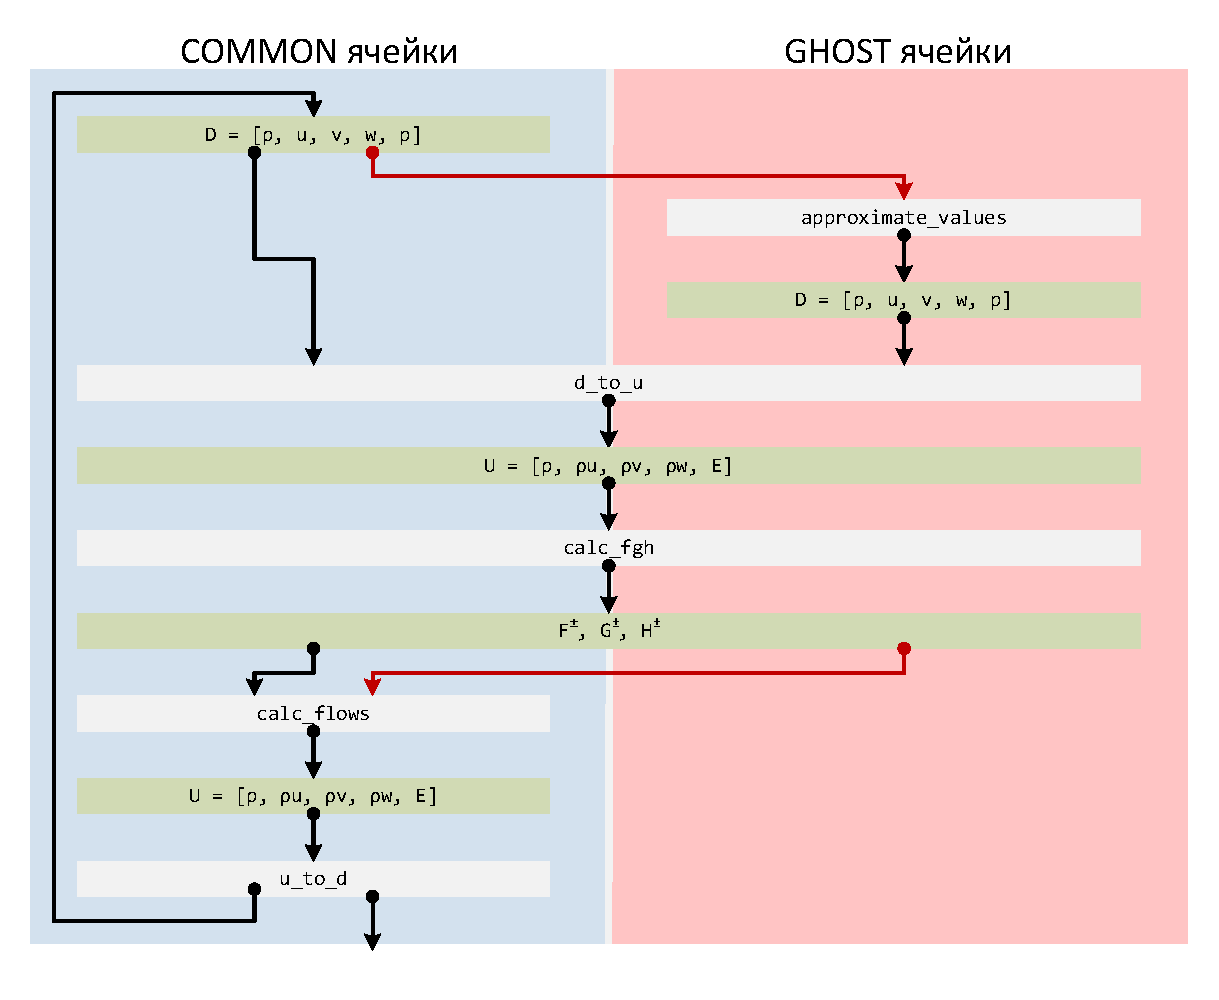
\includegraphics[width=0.6\textwidth]{fig/int_ibm_scheme.pdf}
\singlespacing
\captionstyle{center}\caption{Схема выполнения итерации расчетов методом погруженных границ с использованием схемы Стегера-Уорминга.}
\label{fig:text_4_ibm_immersed_boundary_method_cheme}
\end{figure}

Использование метода погруженных границ с фиктивными ячейками позволяет проводить газодинамические расчеты вблизи сложных границ без необходимости построения согласованных сеток.

%С помощью описанного метода и с применением схемы расчета Стегера-Уорминга были проведены расчеты модельной задачи обтекания свободным потоком множества случайных сфер (при этом граница обтекаемых объектов задавалась аналитически, а не с помощью поверхностной сетки).
%Во время расчетов геометрическая конфигурация оставалась неизменной, что сделало возможным однократное вычисление вспомогательных объектов для аппроксимации газодинамических величин в фиктивных ячейках (в том числе речь идет о матрицах $B_{G123}^{-1}$ и $B_{0'123}^{-1}$ из \eqref{eqn:text_1_ibm_B} и \eqref{eqn:text_1_ibm_B1}).
%С помощью метода погруженных границ на декартовой расчетной сетке можно получить качественно правильную картину обтекания, что проиллюстрировано на рис.~\ref{fig:text_4_ibm_res}.

%\begin{figure}[ht]
%\centering
%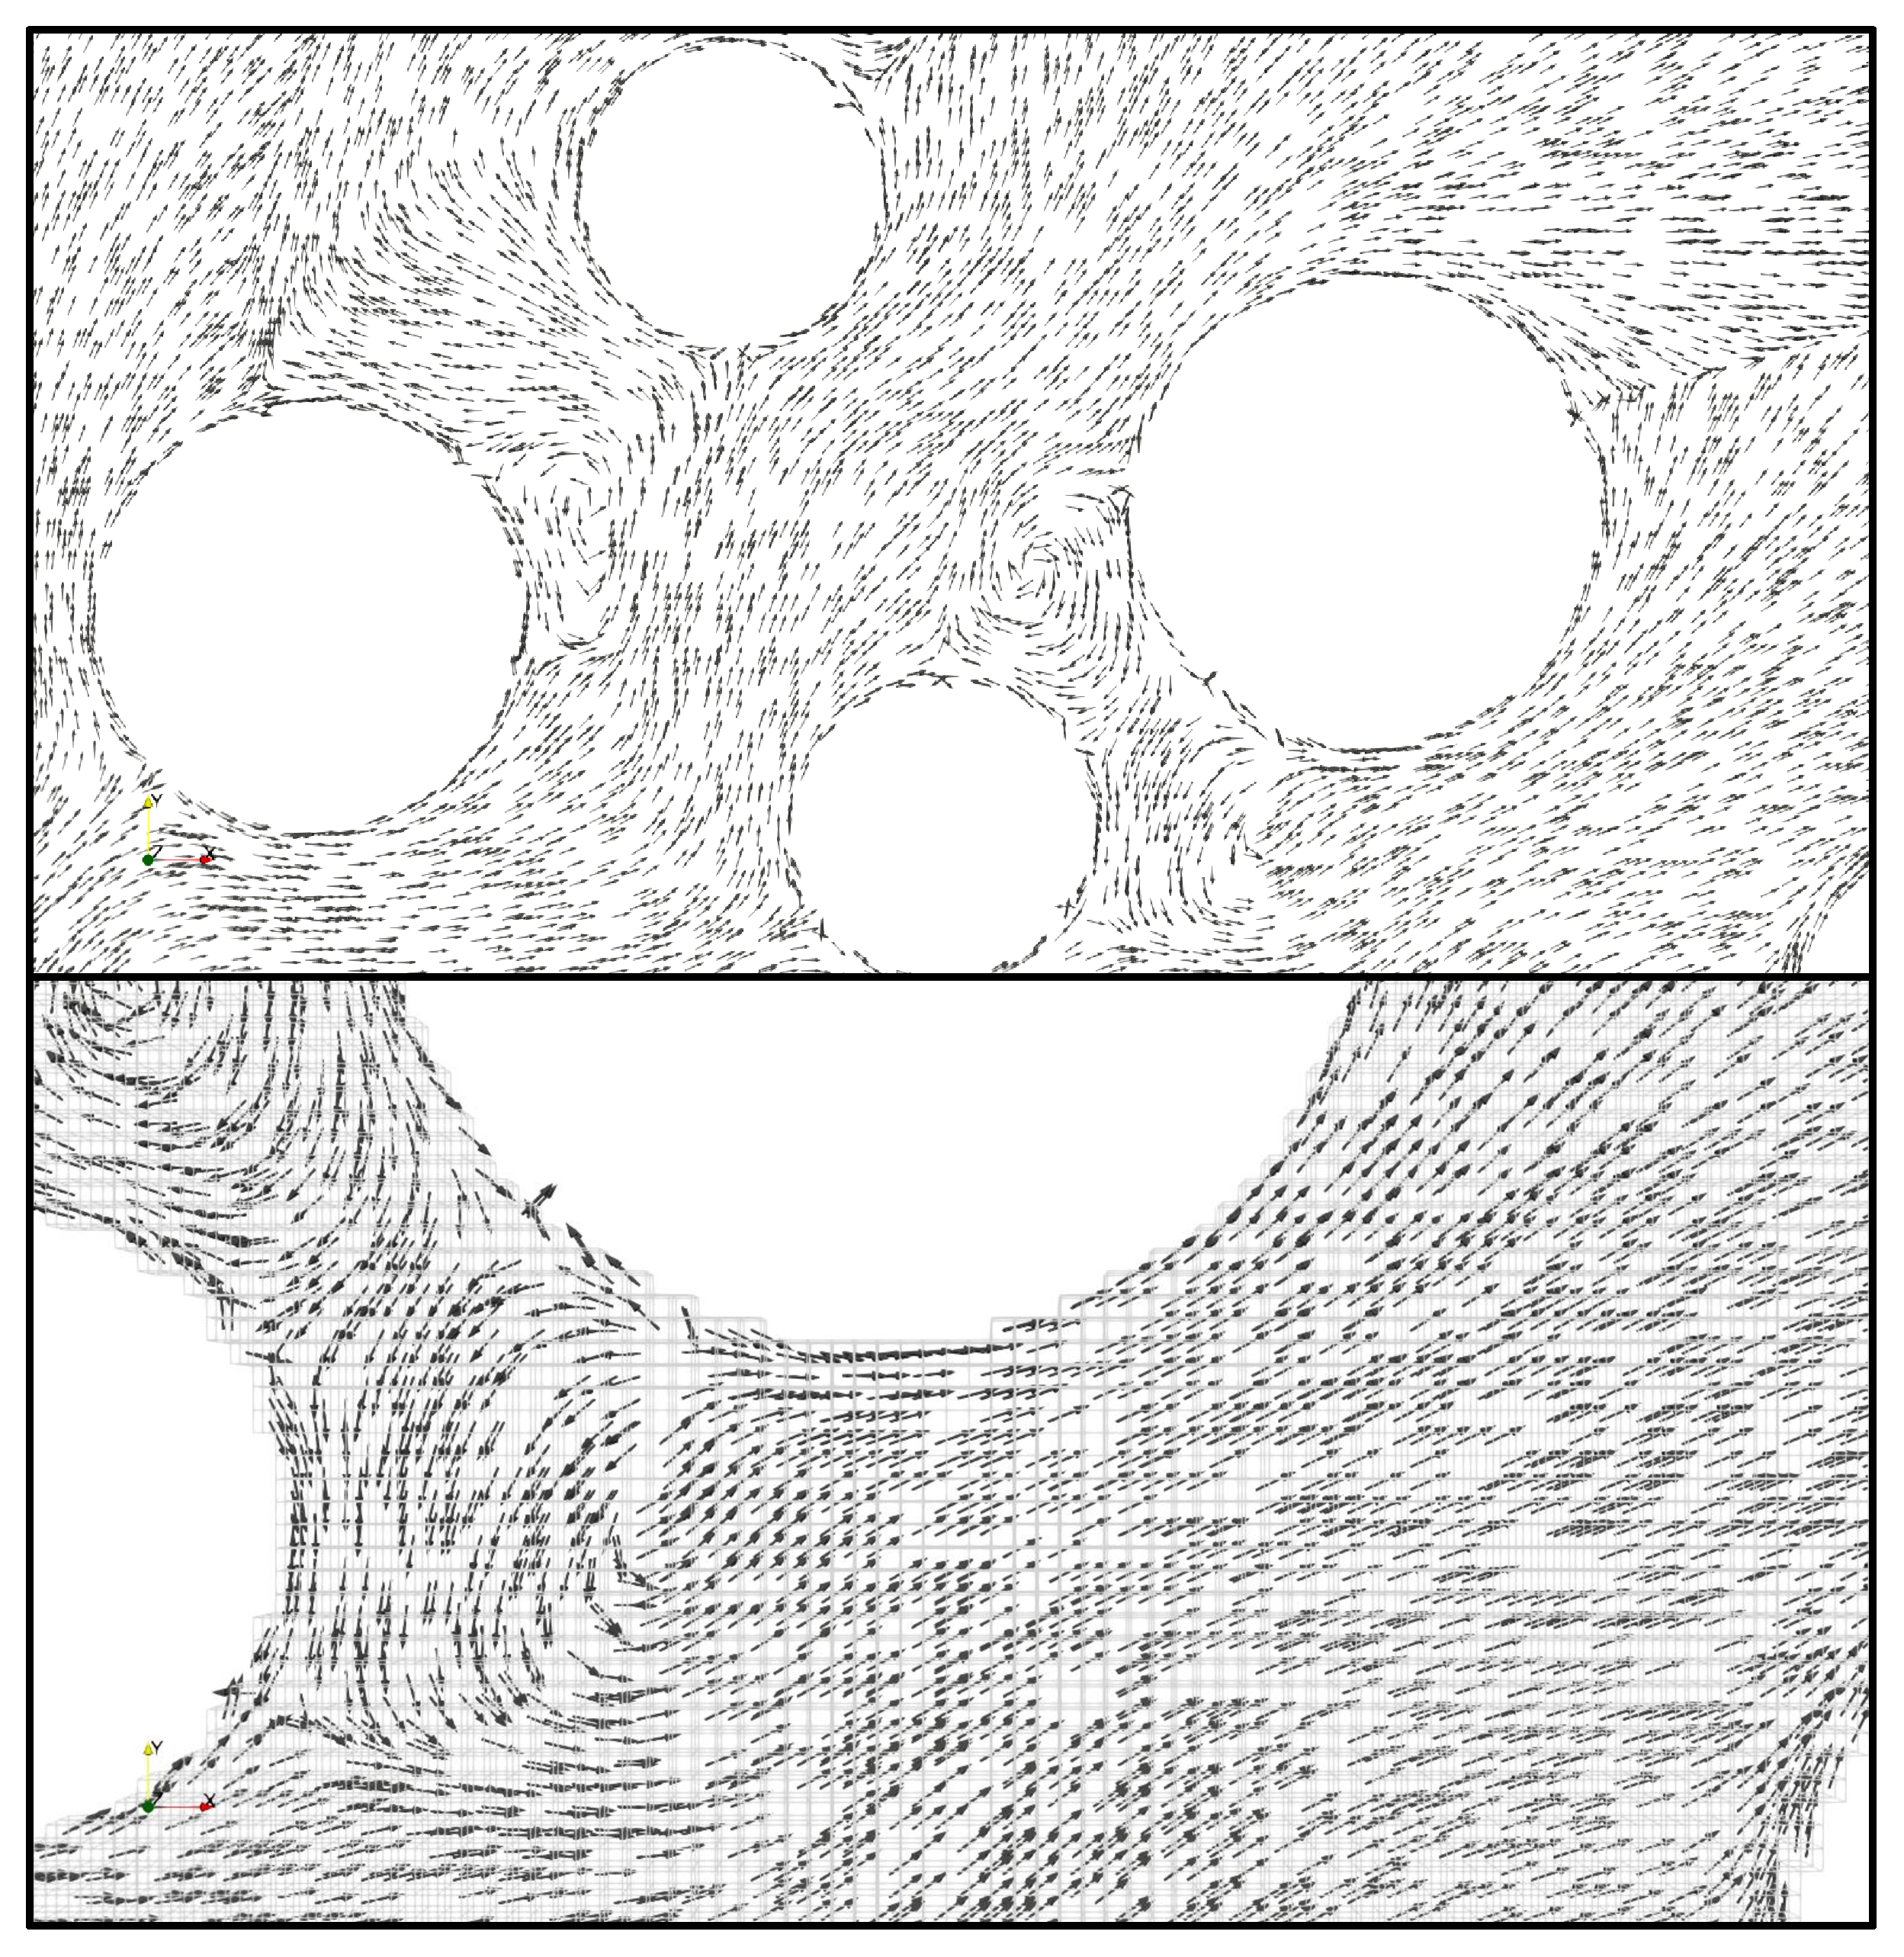
\includegraphics[width=0.8\textwidth]{./pics/text_4_ibm/res.pdf}
%\singlespacing
%\captionstyle{center}\caption{Визуализация поля скоростей (двумерный срез), полученного с помощью метода погруженной границы.}
%\label{fig:text_4_ibm_res}
%\end{figure}

%---------------------------------------------------------------------------------------------------

\subsection{Выводы из главы}

В главе рассмотрены различные методы удаления самопересечений и проанализирована возможность их применения для моделирования ледообразования.
Рассмотрен метод удаления самопересечений с помощью восстановления сетки, который применим только на ограниченном множестве сеток для простых случаев.
Предложен метод удаления самопересечений для замкнутых расчетных сеток с помощью обхода внешней поверхности распространения льда, рассматриваются особенности применениия метода для простых сеток (случай, в котором пересечение двух ячеек возможно только по отрезку, один конец которого лежит внутри одной ячейки, а другой конец -- внутри другой ячейки) и в общем случае с помощью использования рациональных координат.
Предложен метод удаления самопересечений для псевдотрехмерных профилей с помощью сеточной подложки и стягивания расчетной сетки по ребрам.
Предложенные методы удаления самопересечений позволяют позволяют сохранить корректное состояние внешней поверхности области распространения льда при моделировании ледообразования.
Метод поиска пересечения поверхностной сетки с подложкой и предложенный метод погруженной границы для сопряжения с газодинамическим решателем позволяют выполнять расчет поля скоростей без необходимости создания согласованной расчетной сетки в пространстве.

%---------------------------------------------------------------------------------------------------
